% Archivo thesis.tex
% Documento maestro que incluye todos los paquetes necesarios para el documento principal.

% Documento obtenido por un sinfin de iteraciones de administradores del LDC
% Estructura actual hecha por:
% Jairo Lopez <jairo@ldc.usb.ve>
% Actualizado ligeramente por:
% Alexander Tough 

% Definición del documento
\documentclass[oneside,12pt,letterpaper]{report}
\tolerance=1000  
\hbadness=10000  
\raggedbottom

% -- Inicio de la definición de paquetes -- %

% Para escribir algoritmos
\usepackage{listings}
\usepackage{longtable}
\usepackage{pdflscape}

% Paquetes para manejar gráficos
\usepackage{epsf}
\usepackage[pdftex]{graphicx}
\usepackage{epsfig}

% Para más símbolos matemáticos
\usepackage{amsmath}
\usepackage{amsthm}
\usepackage{amssymb}

% Paquetes para presentar una tesis decente.
\usepackage{setspace,cite} % Doble espacio para texto, espacio singular para
                           % los caption y pie de pagina
                           
\usepackage{rotating}
\usepackage{epstopdf}

\usepackage[table]{xcolor}
\usepackage{tikz}
\usepackage{helvet}
\usepackage{float}
%\usepackage{floatrow}
\floatstyle{plaintop}
\restylefloat{table}

%\usepackage{titlesec}
\usetikzlibrary{shapes.geometric,arrows}

\usetikzlibrary{arrows,shapes}
\usepackage{verbatim}

\usepackage{comment}

% Paquetes no utilizados para citas
%\usepackage{mcite} 
%\usepackage{draft} 

\usepackage{wrapfig}
\usepackage{alltt}

% Paquetes para idioma
\usepackage[spanish]{babel}
\usepackage[fixlanguage]{babelbib}
\usepackage[spanish]{translator}
\usepackage[utf8]{inputenc}
\usepackage{color, xcolor, colortbl}
\usepackage{multirow}
\usepackage{subfig}
\usepackage[OT1]{fontenc}
\usepackage{tocbibind}
\usepackage{anysize}
\usepackage{listings} 

% Para poder tener texto asiático
%\usepackage{CJK}
\usepackage{pdfpages}

% Opciones para los glosarios
\usepackage[style=altlist,toc,nonumberlist,acronym]{glossaries}
\usepackage{url}
\usepackage{amsthm}
\usepackage{amsmath}
\usepackage{fancyhdr} % Necesario para los encabezados
\usepackage{fancyvrb}
\usepackage{makeidx} % En caso de necesitar indices.
\makeindex  % Necesitado para los indices

% Definiciones para definiciones, teoremas y lemas
\theoremstyle{definition} \newtheorem{definicion}{Definici\'{o}n}
\theoremstyle{plain} \newtheorem{teorema}{Teorema}
\theoremstyle{plain} \newtheorem{lema}{Lema}

% Para la creación de los pdfs
\usepackage{hyperref}
\hypersetup{urlcolor=blue, colorlinks=false}

% Para resolver el lió del Unicode para la informacion de los PDFs
% En pdftitle coloca el nombre de su proyecto de grado/pasantia.
% En pdfauthor coloca su nombre.
\hypersetup{
    pdftitle = {MÓDULO PARA LA DETECCIÓN DE ATAQUE MEDIANTE BRO},
    pdfauthor={Alejandra Cordero García},
    colorlinks,
    citecolor=black,
    filecolor=black,
    linkcolor=black,
    urlcolor=black,
}


\makeatletter
\newcount\dirtree@lvl
\newcount\dirtree@plvl
\newcount\dirtree@clvl
\def\dirtree@growth{%
  \ifnum\tikznumberofcurrentchild=1\relax
  \global\advance\dirtree@plvl by 1
  \expandafter\xdef\csname dirtree@p@\the\dirtree@plvl\endcsname{\the\dirtree@lvl}
  \fi
  \global\advance\dirtree@lvl by 1\relax
  \dirtree@clvl=\dirtree@lvl
  \advance\dirtree@clvl by -\csname dirtree@p@\the\dirtree@plvl\endcsname
  \pgf@xa=1cm\relax
  \pgf@ya=-1cm\relax
  \pgf@ya=\dirtree@clvl\pgf@ya
  \pgftransformshift{\pgfqpoint{\the\pgf@xa}{\the\pgf@ya}}%
  \ifnum\tikznumberofcurrentchild=\tikznumberofchildren
  \global\advance\dirtree@plvl by -1
  \fi
}

\tikzset{
  dirtree/.style={
    growth function=\dirtree@growth,
    every node/.style={anchor=north},
    every child node/.style={anchor=west},
    edge from parent path={(\tikzparentnode\tikzparentanchor) |- (\tikzchildnode\tikzchildanchor)}
  }
}
\makeatother

\definecolor{brown}{rgb}{0.7,0.2,0}
\definecolor{darkgreen}{rgb}{0,0.6,0.1}
\definecolor{darkgrey}{rgb}{0.4,0.4,0.4}
\definecolor{lightgrey}{rgb}{0.95,0.95,0.95}

\usepackage{listings}
\lstnewenvironment{code}{\lstset{basicstyle=\small}}{}

\lstset{escapeinside=~~}
\lstset{
   frame=single,
   framerule=1pt,
   showstringspaces=false,
   basicstyle=\footnotesize\ttfamily,
   keywordstyle=\textbf,
   backgroundcolor=\color{lightgrey}
}

% Crea el glosario
\makeglossaries

% Incluye el glosario
%\input{apendices/glosario.tex}

% Para crear la hoja escaneada de las firmas
\usepackage[absolute]{textpos}

% Para que no hayan espacios entre items de listas
\usepackage{enumitem} 

% Pone los nombres y las opciones para mostrar los codigos fuentes
\lstset{language=C, breaklines=true, frame=single, showstringspaces=false,
        showtabs=false, numbers=left, keywordstyle=\color{black},
        basicstyle=\footnotesize, captionpos=b }
\renewcommand{\lstlistingname}{C\'{o}digo fuente}
\renewcommand{\lstlistlistingname}{\'{I}ndice de c\'{o}digos fuentes}

\newcommand{\todo}{ TODO: }

% Dimensiones de la pagina
\setlength{\headheight}{15pt}

% Margenes del informe 
\marginsize{3cm}{2cm}{2cm}{2cm}

% Glosario y lista de abreviaturas
\usepackage{longtable}
\usepackage[acronym]{glossaries}
\makeglossaries 
\loadglsentries{./partes/0_abreviaturas.tex}

\usepackage{hyperref}
\usepackage{bookmark}

% Centrar el titulo de los capítulos
\usepackage{titlesec}
\titleformat{\chapter}[display]
  {\normalfont\centering\bfseries}
  {\large\MakeUppercase{\chaptertitlename}~\thechapter}
  {.5em}
  {\MakeUppercase}
  
% Reducir el tamaño de las secciones
\titleformat*{\section}{\normalsize\bfseries}
\titleformat*{\subsection}{\normalsize\bfseries}
\titleformat*{\subsubsection}{\normalsize\bfseries}
\titleformat*{\paragraph}{\normalsize\bfseries}
\titleformat*{\subparagraph}{\normalsize\bfseries}

% -- Inicio del documento 

\begin{document}

% Pagina de titulo
% Pagina de titulo
\begin{titlepage}
\begin{center}

% Upper part (aqui ya esta incluido el logo de la USB).

\includegraphics[scale=0.5,type=png,ext=.png,read=.png]{./img/usb} \\

% Encabezado
\textsc {\large UNIVERSIDAD SIMÓN BOLÍVAR} \\
\textsc{\bfseries DECANATO DE ESTUDIOS PROFESIONALES\\
COORDINACIÓN DE INGENIERÍA DE LA COMPUTACIÓN}

\bigskip
\bigskip
\bigskip
\bigskip
\bigskip
\bigskip
\bigskip
\bigskip
\bigskip

% Title/Titulo
% Aqui ponga el nombre de su proyecto de grado/pasantia larga
\textsc{\bfseries MÓDULO PARA LA DETECCIÓN DE ATAQUE MEDIANTE BRO}

\bigskip
\bigskip
\bigskip
\bigskip
\bigskip

% Author and supervisor/Autor y tutor
\begin{minipage}{\textwidth}
\centering
Por: \\ ALEJANDRA CORDERO GARCÍA\\

\bigskip
\bigskip
\bigskip

\end{minipage}

\bigskip
\bigskip
\bigskip
\bigskip
\bigskip
\bigskip
\bigskip
\bigskip
\bigskip

% Bottom half
{INFORME DE PASANTÍA LARGA \\ Presentado ante la Ilustre Universidad Simón Bolívar \\
como requisito parcial para optar al título de \\ Ingeniero en Computación} \\

\bigskip
\bigskip
\vfill

% Date/Fecha 
{\large \bfseries Sartenejas, 
%FECHA
octubre de 2017}

\end{center}
\end{titlepage}

% Pagina de titulo
\begin{titlepage}
\begin{center}

% Upper part (aqui ya esta incluido el logo de la USB).

\includegraphics[scale=0.5,type=png,ext=.png,read=.png]{./img/usb} \\

% Encabezado
\textsc {\large UNIVERSIDAD SIMÓN BOLÍVAR} \\
\textsc{\bfseries DECANATO DE ESTUDIOS PROFESIONALES\\
COORDINACIÓN DE INGENIERÍA DE LA COMPUTACIÓN}

\bigskip
\bigskip
\bigskip
\bigskip
\bigskip
\bigskip
\bigskip
\bigskip
\bigskip

% Title/Titulo
% Aqui ponga el nombre de su proyecto de grado/pasantia larga
\textsc{\bfseries MÓDULO PARA LA DETECCIÓN DE ATAQUE MEDIANTE BRO}




\bigskip
\bigskip
\bigskip
\bigskip
\bigskip

% Author and supervisor/Autor y tutor
\begin{minipage}{\textwidth}
\centering
Por: \\ ALEJANDRA CORDERO GARCÍA \\

\bigskip
\bigskip
\bigskip

Realizado con la asesoría de: \\
Tutor Académico: PROF. KITY ÁLVAREZ\\
Tutor Industrial: DR. JESÚS VERDEJO DÍAZ
\end{minipage}

\bigskip
\bigskip
\bigskip
\bigskip
\bigskip
\bigskip
\bigskip
\bigskip
\bigskip

% Bottom half
{INFORME DE PASANTÍA LARGA \\ Presentado ante la Ilustre Universidad Simón Bolívar \\
como requisito parcial para optar al título de \\ Ingeniero en Computación} \\

\bigskip
\bigskip
\vfill

% Date/Fecha 
{\large \bfseries Sartenejas, 
%FECHA
octubre de 2017}

\end{center}
\end{titlepage}


% Pagina de acta 1
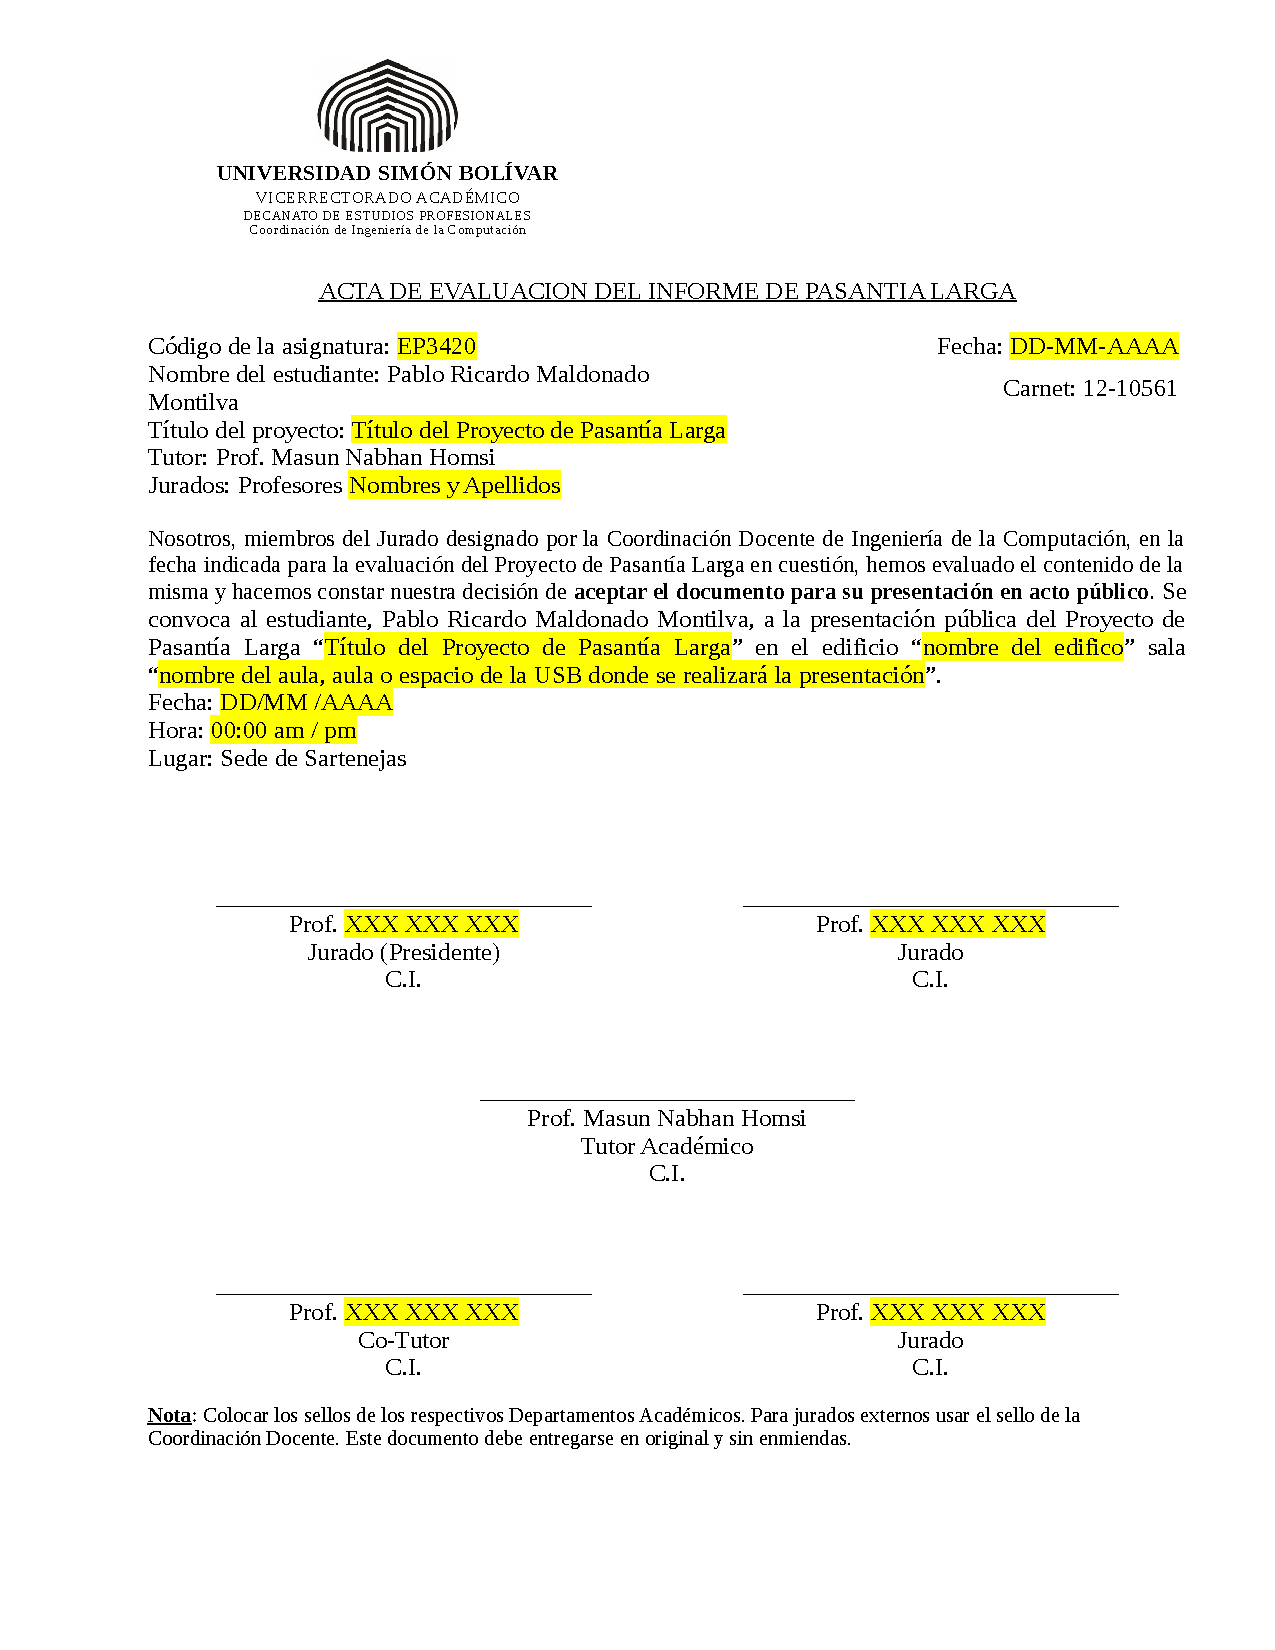
\includepdf[pages={1}]{actas/acta1.pdf}

% Pagina de acta 2
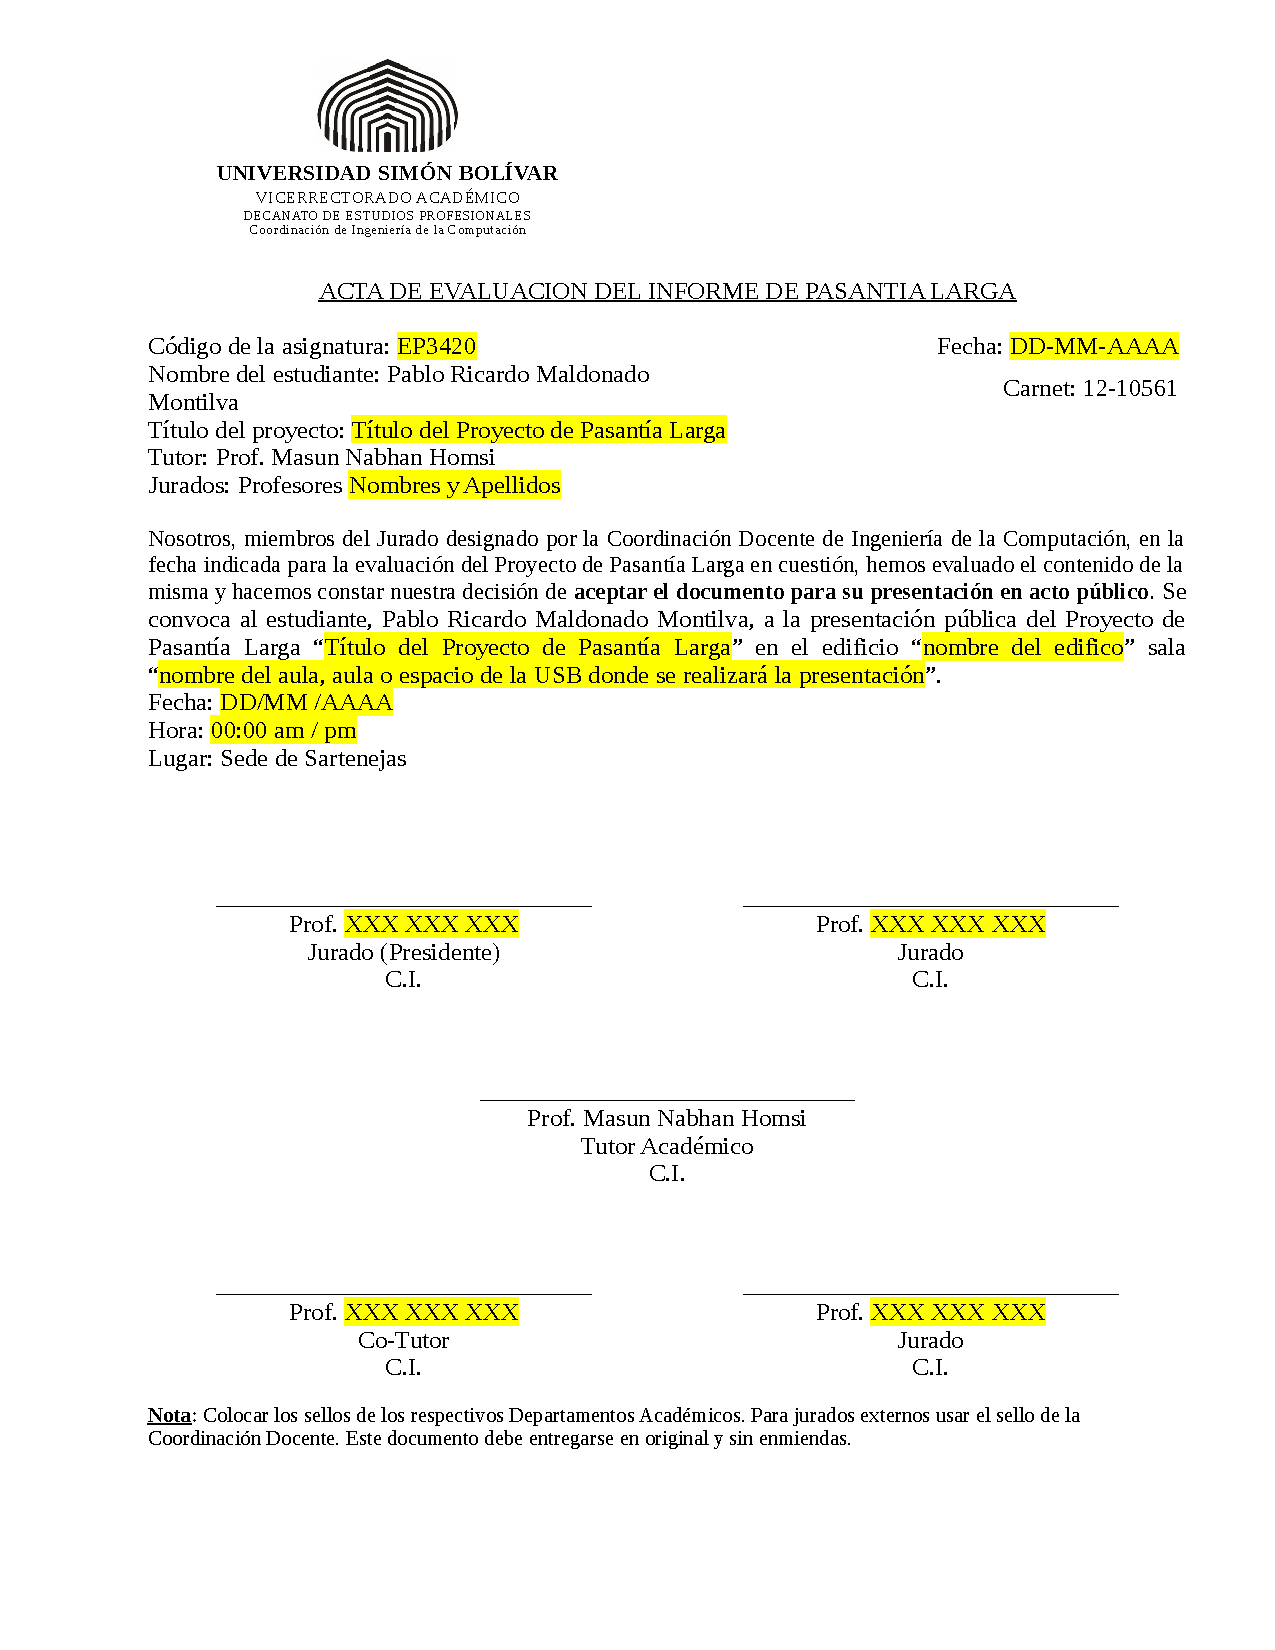
\includepdf[pages={1}]{actas/acta1.pdf}

\setcounter{secnumdepth}{3}
\setcounter{tocdepth}{4}

% Define encabezado números romanos y como se separan los capítulos y las
% secciones
\addtolength{\headheight}{3pt}
\pagenumbering{roman}
\pagestyle{fancyplain}

\renewcommand{\chaptermark}[1]{\markboth{\chaptername\ \thechapter:\,\ #1}{}}
\renewcommand{\sectionmark}[1]{\markright{\thesection\,\ #1}}

\onehalfspacing

\lhead{}
\chead{}
\rhead{}
\renewcommand{\headrulewidth}{0.0pt}
\lfoot{}
\cfoot{\fancyplain{}{\thepage}}
\rfoot{}

% Cambios de titulos de indices
\renewcommand{\listfigurename}{Índice de Figuras}
%\renewcommand{\listtablename}{Índice de Tablas}
%\renewcommand{\tablename}{Tabla}
\renewcommand{\contentsname}{Índice General}
\renewcommand\bibname{Referencias}

% Pagina de resumen
\setcounter{page}{5}
\begin{center}

{\bfseries MÓDULO PARA LA DETECCIÓN DE
ATAQUE MEDIANTE BRO\\}
\bigskip
Por: \\ Alejandra Del Carmen Cordero García\\
\bigskip
\bigskip
{\bf RESUMEN} \pdfbookmark[0]{Resumen}{resumen} % Sets a PDF bookmark for the dedication
\end{center}	

La pasantía larga consistió en desarrollar e implementar los
módulos necesarios para construir un detector de intrusiones para servicios
web, basado en SSM (por el ingles, ``Segmented Stochastic Modelling''),
que se pueda utilizar en redes de explotación. El detector fué implementado
haciendo uso del lenguaje de ``scripting'' de un sistema de monitorización
llamado Bro. Este sistema, se encargará de tomar peticiones HTTP de tipo
GET, extraer sus URIs y analizar si los mismas poseen anomalías de una
manera probabilística, utilizando modelos de normalidad. En el caso en el
que se perciba alguna anormalidad, el sistema se encargará de emitir una
alarma.
El proyecto estuvo dividido en varias fases: La primera fase consistió en
estudiar SSM y sus conceptos relacionados, así como familiarizarse con la
herramienta Bro; la segunda fase se basó en diseñar y dividir las tareas del
sistema en tres módulos principales: un modulo de segmentación, un módulo
de evaluación y un módulo de entrenamiento; en la tercera fase se realizó la
implementación y las pruebas funcionales del detector de intrusiones; en la
cuarta fase se realizaron las pruebas operativas al sistema completo haciendo
uso de bases de datos con trazas normales y bases de datos con trazas
anómalas; y finalmente,en la sexta fase, se estructuró y se redactó la memoria
del proyecto.

% Las palabras clave son generalmente los nombres de áreas de investigación a
% los cuales está asociado el trabajo. Generalmente son tres o cuatro.
\vfill
\textbf{Palabras clave}: SSM, HTTP, GET, URI, Bro.
 

% Pagina de agradecimientos (opcional)
%%\setcounter{page}{6}
\chapter*{Agradecimientos}
\lhead{Agradecimientos}
%\markboth{Agradecimientos}{Agradecimientos}
\pdfbookmark[0]{Agradecimientos}{agradecimientos}
\spacing{1.5}


\bigskip


% Crea la tabla de contenidos
\tableofcontents
% Crea la lista de cuadros
%\listoftables

% Crea la lista de figuras
\listoffigures
\newpage
\phantomsection

% Crea la lista de símbolos

% Crea la lista de códigos fuentes
%\lstlistoflistings

% Crea la lista de abreviaturas
\printglossary[style=list,type=\acronymtype,title=Lista de abreviaturas]


\clearpage

% Define encabezado en números arabicos  
\pagenumbering{arabic}

\fancyhf{} % Redefine el encabezado 
\lhead{}
\chead{}
\rhead{\fancyplain{}{\thepage}}
\renewcommand{\headrulewidth}{0.0pt}
\lfoot{}
\cfoot{}
\rfoot{}

\spacing{1.5}

% Incluye los archivos deseados - El contenido de su proyecto de grado/pasantia larga.
%\phantomsection
%\addcontentsline{toc}{chapter}{Introducción}


\chapter*{Introducción}
\label{intro}
\lhead{\emph{Introducción}}
\addcontentsline{toc}{chapter}{Introducción}


Hoy en dia es muy dif\'icil imaginar el mundo sin el Internet. Esta gran red de redes se ha convertido con el pasar de los años en la espina dorsal del mundo y se estima que mas y mas dispositivos se iran uniendo a esta  en un futuro.

Un gran porcentaje del uso que se le da al Internet proviene de las aplicaciones web. Las aplicaciones web son programas cliente-servidor en donde el cliente se corre en un web browser. Estas pueden ser desde correos electronicos, hasta paginas web con algun servicio en especifico. Para compartir toda la informacion brindada por estas aplicaciones a traves del Internet, se hace uso del protocolo HTTP (Hypertext Transfer Protocol). 
Es aqui donde entran los servidores HTTP, estos servidores son los encargados de suplir las peticiones de sus clientes y enviar o recibir la informacion por los mismos.

Este tipo de servidores son un punto apetecible para los hackers ya que los mismos contienen informacion importante de las aplicaciones web. Como acceso a la base de datos de la aplicacion que contiene las claves, los nombres de usuarios y numero de tarjetas de credito.

Una gran cantidad de informacion esta depositada en servidores de este tipo, es por esto, que es de total importancia velar por su seguridad.

Este tema en cierta medida ser\'a el tema central en el presente trabajo. En el mismo, se hablara sobre la implementación de un protocolo desarrollado por J.E. Díaz-Verdejo, P. García-Teodoro, P. Muñoz, G. Maciá-Fernández, F. De Toro de la Universidad de Granada llamado SSM (Segmented Stochastic Modelling) en un lenguaje se scripting de un analizador de redes llamado Bro.

SSM (Segmented Stochastic Modelling) es un sistema que “se basa en la definición de un autómata de estados finitos estocástico capaz de evaluar la probabilidad de generación de una petición concreta. El autómata permitirá, por tanto, dada una petición, evaluar si dicha petición es legítima (corresponde al modelo) y su probabilidad. En función de la probabilidad y de un umbral se clasificaran las peticiones como normales o anormales” J.E. Díaz-Verdejo, P. García-Teodoro, P. Muñoz, G. Maciá-Fernández, F. De Toro. 2007. Una aproximación basada en Snort para el desarrollo eimplantación de IDS híbridos.

El objetivo de implementar este sistema es el de crear un detector de instrusiones (IDS) que detecte de manera adecuada intrusiones en servidores de tipo HTTP.

En el siguiente trabajo se explicar\'an los detalles de la implementaci\'on del sistema, sus bases te\'oricas y las pruebas realizadas sobre el mismo. La estructura de este ser\'a la siguiente:

En el capitulo uno se hablar\'a sobre la motivación de realizar dicho proyecto, los objetivos tanto generales como especificos, la planificaci\'on que se utilizo para realizar el proyecto y el presupuesto del mismo.

Por otra parte,en el segundo cap\'itulo se tocar\'an temas relacionados con el estado del arte del proyecto.  En primero lugar se explicara la definici\'on de IDS y los tipos de IDS que existen, se explicara la composici\'on de los URI seg\'un el RFC (mencionar el numero del RFC) y se dar\'a una descripci\'on del funcionamiento SSM los modelos que lo conforman. Adem\'as, se hablar\'a sobre la herramiento utilizada y el lenguaje de scripting se utiliz\'o para implementar el sistema.

En el tercer capitulo se hablara sobre el diseño del sistema. Aqu\'i se describir\'an los modulos en los que esta dividido el IDS y como es el funcionamiento de cada uno. Los detalles de implementacion de estos se explicaran en el capitulo cuarto.

El quinto capitulo tocar\'a el tema de la evaluaci\'on y las pruebas. En este capitulo se hablara sobre la base de datos utilizada para realizar las pruebas y los resultados arrojados por las mismas. Adem\'as se describiran un poco las pruebas tanto operativas como funcionales realizadas sobre el sistema.

% Descripción del problema, de lo general hacia lo específico


% Trabajos anteriores


% Objetivo general


% Objetivos específicos

% Organización del trabajo
% Se describe brevemente qué se hace en cada capítulo


%\chapter{El Problema}
\label{capitulo1}

% De qué va a tratar el capítulo
% El capítulo 1 suele ser el marco teórico.
\section{Planteamiento del Problema}

Internet con el pasar de los años se ha estado integrando cada vez más en varios aspectos de las vidas. A pesar de todos los beneficios que trae estar conectados a esta red de redes, es preciso recalcar igualmente los problemas que acarrea el hecho de estar enlazados a esta sin la existencia de medidas de seguridad necesarias. 

Los dispositivos, las aplicaciones y los sistemas que utilizamos en el día a día almacenan información valiosa a la que pueden acceder personas no deseadas si no existen las medidas necesarias en las redes para evitar los ciberataques. Cada día más y más información digital existe en el mundo, y mientras crece el volumen de dicha información , aumenta también la cantidad de ciberataques que se realizan \cite{pwc}. Es por esta razón, que el concepto de ciberseguridad es de vital importancia cuando hablamos del cibermundo.  La ciberseguridad, se encarga de proteger redes de comunicación, sistemas y datos de ataques cibernéticos. 

Uno de los métodos utilizados en la ciberseguridad son los detectores de intrusiones (IDS, por sus siglas en inglés ``Intrusion-detection system''). Un IDS es detector que procesa información proveniente del sistema o redes de computadores que se desea proteger. Una vez que que detectada una intrusión este lanza alertas para activar el proceso de auditoría por parte de los administradores de sistema \cite{IDS}. 

Por otra parte, uno de los servicios más utilizados en el mundo del Internet y que más contienen información son los servicios web. Estas características hacen que este tipo de servicios sea uno de los más apetecibles para los ciberataques. Se hace evidente entonces, que se requieren medidas en el área de la ciberseguridad dirigidas a estos casos.

Es por esta razón que grupos de investigación se han dedicado a tratar de solventar dicho problema. Tal es el caso del grupo de investigación de la Universidad de Granada que  ha desarrollado un IDS para detectar ataques a servidores web llamado SSM (``Segmented Stochastic Modelling'') y así evitar problemas como: el reconocimiento, el escaneo de paquetes de red, la obtención y el mantenimiento de acceso al servidor y la modificación de ``logs'' que evitan que se rastree el ataque en este tipo de servicios.

Es por ello que resultaría interesante implementar un sistema de intrusiones que ha presentados resultados satisfactorios como es el caso de SSM haciendo uso de una herramienta tan potente y en auge como lo es Bro.

\section{Objetivos}
\subsection{Objetivos Generales}
El objetivo del presente trabajo es incorporar la técnica de detección de intrusiones SSM propuesta en \cite{ssm} en el sistema Bro. Para ello deben usarse las capacidades de ``scripting'' de Bro e incorporar las funcionalidades necesarias como un módulo que pueda activarse a demanda para monitorizar las peticiones a los servicios web.
\subsection{Objetivos Específicos}
La consecución del objetivo general planteado puede abordarse a partir de los siguientes objetivos específicos:

\begin{enumerate}
\item Interceptar las URI para su análisis haciendo uso de Bro para capturar y filtrar la información de los paquetes del protocolo HTTP.
\item Desarrollar un módulo que permita evaluar el índice de anomalía de los URI haciendo uso de las herramientas otorgadas por el lenguaje de ``scripting'' de Bro y siguiendo las especificaciones y expresiones pautadas por la técnica de detección de intrusiones SSM. 
\item Desarrollar un módulo para la estimación de los modelos de normalidad haciendo uso de las herramientas otorgadas por el lenguaje de ``scripting'' de Bro que permita obtener un modelo de normalidad a partir de trafico libre de ataques.
\item Evaluar experimentalmente el funcionamiento del sistema realizando pruebas, tanto funcionales como operativas para verificar el correcto funcionamiento del mismo.
\end{enumerate}

\section{Justificación e Importancia}


La intención del proyecto es implementar un detector de intrusiones para servicios web, basado en SSM haciendo uso de la herramienta Bro.

Un Detector de Intrusiones (IDS) es un sistema que monitoriza todas las actividades de un sistema en específico para detectar intrusiones\cite{IDSdef}. Si el mismo detecta una intrusión, se generará una alerta para que los administradores del sistema se encarguen de la misma.

Sin embargo, una pregunta válida que se puede realizar es : ¿Para qué molestarse en instalar un IDS si se tiene un ``firewall'', filtro de ``spam'' y contraseñas de autenticidad? La respuesta es simple: porque las intrusiones siguen ocurriendo. Así como las personas algunas veces olvidan cerrar las ventanas, por ejemplo, también olvidan actualizar el conjunto de reglas del ``firewall''. \cite{IDSimportance}

Es por esto, que los IDS conforman un aspecto importante dentro de la seguridad, ya que si alguno de los elementos fallan siempre estará el detector de intrusiones para generar alertas sobre posibles ataques.

Por otra parte, SSM es un sistema basado en el uso de modelos realizados a partir de las peticiones hechas al servicio web. Los resultados experimentales en este sistema muestran la eficacia del mismo detectando anomalías en este tipo de servicios. Sin embargo, la implementación disponible de SSM es de laboratorio y funciona sobre trazas estáticas, por lo que la técnica no está disponible actualmente para su uso en redes en explotación.

No obstante, para realizar una implementación de sistema que funcione en redes en explotación, se requieren de herramientas aptas que permitan capturar y analizar el tráfico en la red. Por su parte, Bro, es un sistema de monitorización de red de código abierto muy utilizado hoy en día para el desarrollo de mecanismos de seguridad que posee: su propio lenguaje de ``scripting'' y una comunidad de asistencia que va creciendo cada vez más con el tiempo.

Por lo tanto, implementar una técnica que ha tenido resultados satisfactorios como lo es SSM, haciendo uso de Bro, que es una herramienta en auge en el ámbito de la seguridad de redes hoy en día resulta de mucha utilidad ya que esta unión permitirá de manera satisfactoria detectar intrusiones en los servicios web en producción para de esta manera alertar sobre ataques de reconocimiento, escaneo, la obtención y el mantenimiento de acceso al servidor y la modificación de ``logs'' que evitan que se rastree el ataque.


\section{Planificación}

La tareas en las que se divide el desarrollo de este proyecto fueron las siguientes:

\newlist{legal}{enumerate}{10}
\setlist[legal]{label*=\arabic*.}

\begin{legal}
\item Estado del arte

Durante esta etapa se realizará un estudio sobre los IDS, los tipos de IDS y el sistema SSM. Así mismo, se hará una lectura del RFC 3986 (URI) y se investigará sobre el protocolo HTTP.

\item Análisis de Bro

Durante esta etapa del proyecto se instalará, se estudiará la documentación y se aprenderá a hacer uso de la herramienta Bro y su lenguaje de ``scripting''.

\item Arquitectura modular del sistema 

En esta etapa se realizará el diseño de los módulos principales que conforman el sistema. Esta tarea se basará en dividir el trabajo de cada uno de los módulos en varias funcionalidades y en diseñar las estructuras de datos y el formato de los archivos de texto del sistema.

    Esta tarea estará subdividida en las siguientes subtareas:

\begin{legal}
\item Diseño del módulo de análisis sintáctico/segmentación de URIS 
\item Diseño del módulo de evaluación de URIs 
\item Diseño del módulo de entrenamiento 
\end{legal}
\item Implementación del sistema

En esta etapa del proyecto se llevará a cabo la implementación del sistema haciendo uso del lenguaje de ``scripting'' de Bro.

\begin{legal}
\item Módulo de análisis sintáctico/segmentación de URIS 

En esta etapa se tomarán los diseños esbozados previamente y se implementarán todas las funcionalidades necesarias para realizar el segmentador y el analizador sintáctico de los URIS.

\item Módulo de evaluación de URIs 

En esta etapa  se implementarán todas las expresiones, las estructuras de datos y las funcionalidades necesarias para construir un modulo de evaluación funcional haciendo uso de las herramientas presentadas por Bro. 

\item Módulo de entrenamiento 

En esta etapa se implementarán las estructuras de datos y módulo de entrenamiento.

\item Módulo de gestión del tipo de sistema

En esta etapa del proyecto se implementará el módulo de gestión del tipo de sistema haciendo uso de ``bash scripting''. 

\item Módulo de reportes

En esta etapa se implementarán los reportes del sistema haciendo uso de herramientas de Bro dedicadas exclusivamente a realizar este tipo de tareas.

\end{legal}
\item Evaluación y pruebas 

Durante el desarrollo del proyecto se realizarán pruebas funcionales y una vez finalizada la implementación del sistema se procederá a realizar pruebas operativas.
\begin{legal}
\item Realización de pruebas funcionales

Se harán pruebas de manera individual a cada una de las funciones más importantes de los módulos que conforman el sistema y se realizarán las modificaciones pertinentes en las mismas.

\item Realización de pruebas operativas

La realización de las pruebas operativas se basará en tomar base de datos de trazas tanto normales como anormales, probar el funcionamiento de todo el sistema y realizar las modificaciones pertinentes.

\end{legal}

\item Documentación  
 Esta fase consistirá en estructurar y redactar la memoria del proyecto.
\end{legal}

\begin{table}[tb]
\begin{center}
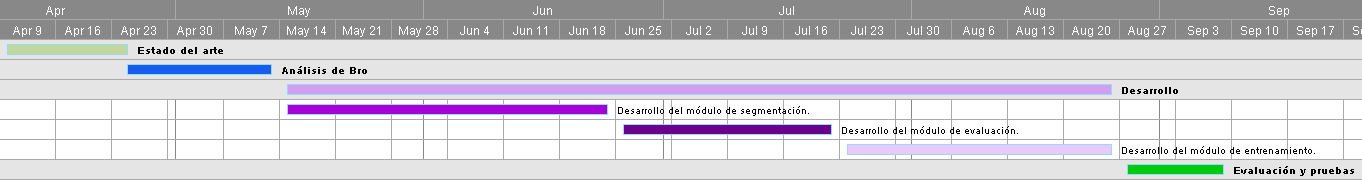
\includegraphics[width=6in]{./img/pasantia.png}
\caption{Diagrama de Gantt del proyecto.}\label{fig1}
\end{center}
\end{table}

\chapter{Entorno Empresarial}
\label{capituloEmpresa}
\section{Descripción de la Empresa}
\section{Misión}
\section{Visión}
\section{Estructura Organizacional}
\section{Organigrama}



\chapter{MARCO TEÓRICO}
\label{capitulo2}
\lhead{Capítulo 2. \emph{Marco teórico}}


En el cap\'itulo se describir\'an algunos conceptos importantes para comprender la implementaci\'on del sistema  en el que se basa el presente trabajo. Dichos conceptos son: \textit{IDS, el protocolo HTTP, URI , autom\'atas de estados finitos, autom\'atas probabilísticos, modelo de Markov,SSM y Bro}.

En l\'ineas generales, se tiene como prop\'osito explicar el funcionamiento de un \textit{IDS} basado en anomalías que haga uso del sistema \textit{SSM} y del lenguaje de scripting de la herramienta \textit{BRO}.

Este sistema analiza los \textit{URI} de las peticiones tipo GET o HEAD del protocolo \textit{HTTP}, haciendo uso de la t\'ecnica \textit{SSM}. Esta t\'ecnica, a su vez hace uso de \textit{autómatas de estados finitos probabilísticos} y del \textit{modelo de Markov} para determinar si las peticiones realizadas a un servidor \textit{HTTP} son posibles ataques o no.
% De qué va a tratar el capítulo
% El capítulo 1 suele ser el marco teórico.

\section{Protocolo HTTP}

El protocolo HTTP, (``Hypertext Transfer Protocol'') es un protocolo de la capa de aplicación que se encuentra en el corazón de la Web. Se define en [RFC 1945] y [RFC 2616]. HTTP esta implementado en dos programas: un programa cliente y un programa servidor. El programa cliente y el programa servidor se ejecutan en diferentes sistemas y se comunican entre si intercambiando mensajes HTTP. HTTP por su parte, define la estructura de dichos mensajes y como se realiza el intercambio de los mismos. \cite{httpKross}

El protocolo HTTP, es un protocolo simple de petición-respuesta que funciona normalmente sobre la capa de transporte TCP. La idea general de la interacción entre el cliente y el servidor se muestra en la figura \ref{fig:httpPeticionRespuesta}. 

\begin{figure}[tb]
\begin{center}
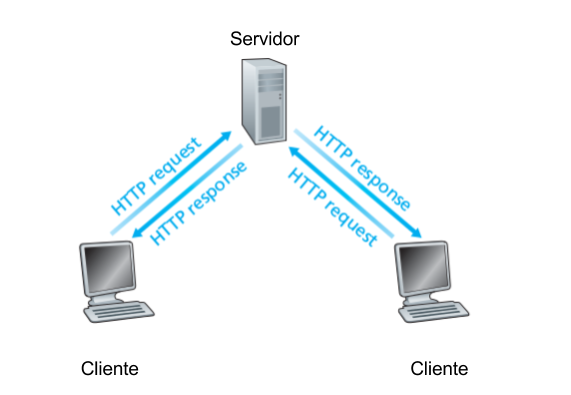
\includegraphics[width=3in]{HTTP.png}
\caption{Petición-respuesta.\cite{httpKross}}
\label{fig:httpPeticionRespuesta}
\end{center}
\end{figure}

En el protocolo HTTP, el cliente inicia la conexión TCP con el servidor. Una vez establecida la conexión, ambos podrán enviar y recibir mensajes de petición y respuesta. La información que se transfiere mediante este protocolo pueden ser archivos de texto plano, hipertexto, audio, imágenes o cualquier información accesible por Internet.

Es importante tener en cuenta que el servidor envía los archivos solicitados a los clientes sin almacenar información del estado de los mismo, es decir, el servidor no almacena información de sus clientes. Debido a esto se dice que HTTP es un protocolo sin estado.\cite{httpKross}

Por otra parte, los mensajes de petición y respuesta del protocolo HTTP poseen una estructura general como la que se muestra en la figura \ref{fig:httpMensaje}.

\begin{figure}[tb]
\begin{center}
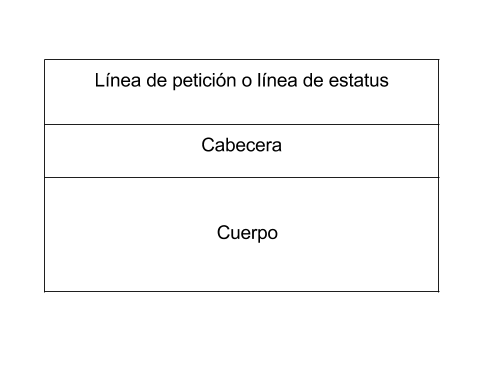
\includegraphics[width=3in]{mensajeHTTP.png}
\caption{Mensaje HTTP.\cite{httpKross}}
\label{fig:httpMensaje}
\end{center}
\end{figure}

La linea de petición en los mensajes HTTP, presenta tres partes separadas por espacios:

\begin{enumerate}
\item El método.
\item El identificador del recurso solicitado (URI).
\item La version del protocolo HTTP.
\end{enumerate}

El método es un parámetro que indica lo que actualmente se esta solicitando por el mensaje. 
Los m\'etodos GET, HEAD y POST son los más utilizados en las comunicaciones del protocolo HTTP. 

\begin{itemize}
\item GET se encarga de hacer solicitudes de recursos al programa servidor HTTP.
\item HEAD solicita recursos de la misma forma en la que lo hace el método GET con la \'unica diferencia de que la solicitud solo ser\'a respondida con la cabecera del recurso, excluyendo el cuerpo del mismo.
\item POST solicita que el recurso de destino  procese la informaci\'on que viene incluida en la solicitud realizada
\end{itemize}

Para el presente trabajo la sintaxis de los URI y los mensajes de petición de tipo GET resultan de importante relevancia.

\section{URI} \label{URIsection}

Un URI es una serie de caracteres que identifican un recurso en la red. Este posee una sintaxis específica que está conformada por diferentes segmentos de caracteres: el esquema, la autoridad, la ruta, el ``query'' y el ``fragment''.

En la figura \ref{fig:URI}, se muestra, en un ejemplo de los componentes que forman un URI.

\begin{figure}[tb]
\begin{center}
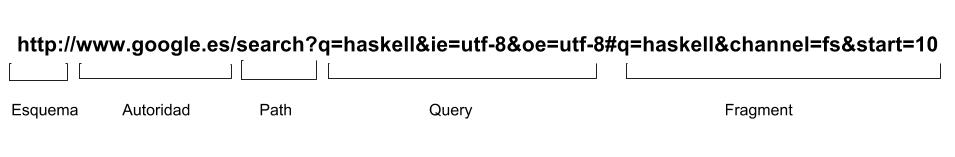
\includegraphics[width=4in]{./URI.jpg}
\caption{URI.}
\label{fig:URI}
\end{center}
\end{figure}

A continuaci\'on se describe de manera breve cada uno de los componentes que pueden conformar un URI.

\begin{itemize}

\item Esquema:

El esquema identifica el protocolo. En el caso del presente trabajo, los URIs utilizaran únicamente el protocolo http o https.


\item Autoridad:

Este componente del URI posee información del ``host'' del URI, el cual viene representado bien sea por un IPv4 o un nombre de dominio, seguido de un número de puerto (opcional).
   
\item ``Path'':
La ruta de un URI es un conjunto de segmentos organizados de manera jerárquica que contienen información sobre la ubicación de los recursos a solicitar.

\item ``Query'':

El ``query'' de un URI es un segmento de información no jerarquizada, cuyo símbolo de inicio es el signo de interrogación (?). Por lo general, el ``query'' está conformado por una dupla ``atributo=valor'' que junto con la ruta identifican el recurso que se desea solicitar. A diferencia de la ruta, la información aquí contenida debe ser procesada por el servidor al que se le está solicitando el recurso. 

\item ``Fragment'':

En un URI, el ``fragment'' corresponde a la dirección de un segundo recurso dentro del primer recurso identificado por la ruta y el ``query''. Esta cadena de caracteres esta precedida por el símbolo de un numeral (\#).

\end{itemize}

En un URI, tanto el esquema como la ruta son segmentos que deben existir de manera obligatoria. Si la ruta es un carácter vac\'io, se asumir\'a que la misma es ``/''. El resto de los segmentos son opcionales.

\section{Detector de intrusiones (IDS)}
Un detector de intrusiones (IDS del inglés "Intrusion-detection system" ) es un sistema que se encarga de procesar la información entrante de un sistema a proteger con la intención de detectar actividades maliciosas y lanzar alertas para activar el proceso de auditoría por parte de los administradores de sistema \cite{IDS}

Los IDS suelen clasificados en: IDS basados en firmas o 		IDS 	basados en anomalías. 

Los IDS basados en firmas, utilizan una base de datos de ataques conocidos y vulnerabilidades del sistema los cuales son utilizados para realizar comparaciones con los patrones seguidos por las actividades detectadas. Si se detecta similitud con alguno de los patrones de la base de datos, se activará una alarma para indicar que un ataque esta siendo perpetuado.

La eficacia de los detectores de intrusiones basados en firmas es muy buena, sin embargo, su buen funcionamiento depende completamente de la constante actualización de la base de datos de ataques.

Por otra parte, los IDS basados en anomalía detectan los ataques de manera diferente. En este tipo de IDS los ataques son detectados a partir de la observación de comportamientos, bien sea del sistema, o de los usuarios. 

El modo de funcionamiento de un IDS basado en anomalía se basa en: recolectar la información de las actividades detectadas y comparar dicha información con un modelo de normalidad del sistema que ha sido previamente construido. El modelo de normalidad se construye a partir de comportamientos previamente observado en el sistema y que son catalogados como "normales". Si existe una incongruencia entre la información entrante y el modelo de normalidad, entonces se generará una alarma.

No obstante, uno de los problemas de este tipo de detector de intrusiones es la alta tasa de falsos positivos que puede llegar a tener. Esto se debe, a que los modelos, por lo general, no contienen todos los comportamientos normales de un sistema en su totalidad. Esto, a su vez provoca que existan eventos libres de ataques que sean catalogados como una amenaza. Tambi\'en está el hecho de que es muy posible que con el pasar del tiempo, el comportamiento del sistema a proteger vaya cambiando, lo cual implicar\'ia que, si no se hace una constante revis\'on y reentrenamiento del modelo de normalidad el mismo quedar\'a obsoleto y los eventos entrante ser\'an mal catalogados por el IDS. El problema de realizar entrenamientos constantes para actualizar un modelo de normalidad es que se crearán brechas de tiempo en donde el sistema ser\'a muy vulnerable a ataques ya que en lugar de estar funcionando el módulo para detección, estar\'a funcionando el módulo para entrenar el modelo de normalidad. Por lo tanto, si un ataque es perpetrado durante ese periodo de tiempo, el mismo quedar\'a grabado en el modelo de normalidad como un comportamiento normal del sistema.

También existen los IDS híbridos cuyo funcionamiento mezcla el funcionamiento de los detectores de intrusiones basados en firmas y los basados en anomalía, es decir, este tipo de  IDS suelen contar con una base de datos de firmas y también con un modelo de normalidad.

\section{Autómatas de estados finitos}

Un autómata es un modelo abstracto de un ordenador digital \cite{automata}. Una manera de definirlo de forma gráfica es como se muestra en la figura \ref{fig:automata}.

\begin{figure}[tb]
\begin{center}
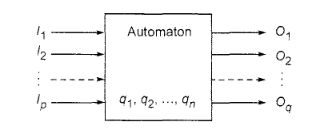
\includegraphics[width=3in]{automata.png}
\caption{Autómata.\cite{automata2}}
\label{fig:automata}
\end{center}
\end{figure}

donde \cite{automata2}:

\begin{itemize}
\item  $I_{1}, I_{2},..., I_{n}$ es el "input" del autómata  que es introducido en cada instante de tiempo $t_{1}, t_{2},..., t_{n}$.

\item $O_{1}, O_{2},..., O_{n}$ es la salida del autómata.

\item $q_{1}, q_{2},..., q_{n}$ son los estado en los que puede estar el autómata en cualquier instante de tiempo.
\end{itemize}

Dentro de los autómatas existe la familia de los autómatas de estado finito. Un autómata de estado de autómata finito se puede definir formalmente como una quíntupla \cite{automataFinito}:.

\begin{equation}
M = (Q,\Sigma,\delta,q,F)
\end{equation}

donde:

\begin{itemize}

\item Q es un conjunto finito de estados.

\item  $\Sigma$ es un conjunto finito, llamado alfabeto. Los elementos de $\Sigma$ se llaman símbolos.

\item $\delta$ es una función de transición, tal que $ Q x \Sigma \leftarrow Q$
 
\item  q  es un elemento perteneciente a Q llamado estado inicial.

\item F es un subconjunto de Q y representa el conjunto de estados finales.

\end{itemize}

Los autómatas finitos se clasifican en autómatas finitos deterministas (DFA, del inglés "Deterministic Finite Automata") y no-deterministas (NFA, del inglés "Nondeterministic Finite Automata").

Los autómatas finitos deterministas se definen teóricamente de la misma manera en la que se definen los autómatas finitos. Sin embargo, se debe cumplir que por cada estado $"s"$ y símbolo de entrada $"a"$ debe existir un único estado al que se puede hacer una transición. Esto quiere decir que la función de transición $\delta$ de los autómatas finitos deben retornar un solo elemento.

Por otra parte, los autómatas finitos no-deterministas al igual que los autómatas finitos deterministas se definen teóricamente de la misma forma que los autómatas finitos. No obstante, la función de transición $\delta$ de estos autómatas puede retornar un conjunto de elementos, es decir, por cada estado $"s"$ y símbolo de entrada $"a"$ pueden existir varios estados al los que se puede hacer una transición.

Tanto los autómatas finitos deterministas como los no deterministas se puede representar a tráves de un grafo. En donde los estados serian representados a tráves de los nodos y las aristas representarían las funciones de transición. 

Un ejemplo de un NFA representado a tráves de un grafo se presenta en la figura \ref{fig:NFA}.

\begin{figure}[tb]
\begin{center}
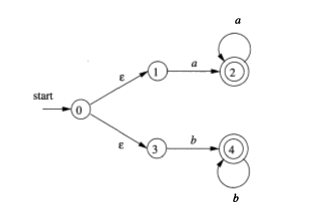
\includegraphics[width=3in]{NFA.png}
\caption{Autómata no-determinista.\cite{automataFinito}}
\label{fig:NFA}
\end{center}
\end{figure}

En la figura \ref{fig:DFA} se muestra la representación de un DFA haciendo uso de un grafo.

\begin{figure}[tb]
\begin{center}
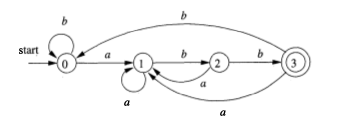
\includegraphics[width=3in]{DFA.png}
\caption{Autómata determinista.\cite{automataFinito}}
\label{fig:DFA}
\end{center}
\end{figure}

Los autómatas deterministas permitirían determinar, dado un autómata asociado a un protocolo, si una secuencia de mensajes intercambiados puede ser decodificada mediante dicho autómata. Esto es, si la secuencia de mensajes corresponde a la especificación del protocolo y, por lo tanto, es gramaticalmente correcta. No obstante, una parte importante de los ataques son estructuralmente correctos de acuerdo al protocolo, es decir, siguen la gramática \cite{tesisMexico}.

Sin embargo, los autómatas no deterministas permitirán discriminar ataques cuya estructura sintáctica sea correcta porque permiten incorporar información relacionada con la semántica o el contexto .

Un tipo de autómata no determinista de especial interés para los objetivos del presente trabajo son los autómatas de estado finitos probabilístico [Brookshear, 1989]. En estos se consideran probabilidades asociadas a los estados y/o a los símbolos de forma que se atribuye una naturaleza probabilística tanto a la secuencia de estados que sigue el sistema como a la de los símbolos observados.


\section{Modelo de Markov}

En un proceso de Markov un evento en un tiempo determinado, depende de los procesos inmediatos anteriores a este \cite{markov}. Un modelo de Markov discreto, por otra parte, consiste en un conjunto de estados y una serie de probabilidad de transición que rigen las transiciones entre estados y la producción de símbolos.

Un modelo de Markov discreto, $\lambda$, se define como un quíntupla:

\begin{equation}
\lambda = (Q,\Theta,A,B,\Pi)
\end{equation}

donde:
 
\begin{itemize}
\item Q :  Es el conjunto de N estados del modelo.
\item $\Theta$ : Es el vocabulario del modelo, es decir, son los posibles s\'imbolos o eventos observables del sistema.
\item A : Es una matriz NxN de probabilidades de transici\'on entre estados.
\begin{equation}
\begin{aligned}
A = [a_{ij}], 1\leq i \leq N  y  1\leq j \leq N.\\
a_{ij} = P(q_{t} = S_{j} | q_{t-1} = S_{i})
\end{aligned}
\end{equation}

\item B : Es una matriz NxM de probabilidades de generaci\'on u observación de los s\'imbolos .
\begin{equation}
\begin{aligned}
B = [b_{ik}], 1\leq i \leq N, 1\leq k \leq M.\\
b_{ik} = P(O_{t} = v_{k} | q_{t} = S_{i})
\end{aligned}
\end{equation}

\item $\Pi$ es el vector de probabilidades del estado inicial.
\begin{equation}
\begin{aligned}
\Pi = [\Pi_{i}], 1\leq i \leq N \\
\pi_{i} = P(q_{1} = S_{i})
\end{aligned}
\end{equation}

\end{itemize}

Un ejemplo sencillo de un modelo de Markov sería el siguiente \cite{ejemploMarkov}

S = {$s_{1}$,$s_{2}$}, donde, $s_{1} = "lluvioso"$ y $s_{2} = "soleado"$ y la matriz de transición es:

\[
 P = \begin{pmatrix}
  0.75 & 0.25  \\
  0.25 & 0.75  \\
 \end{pmatrix}
\]

Un modelo de Markov es un autómata de estados finitos no determinista que puede ser representado mediante grafos.

El ejemplo presentado con anterioridad, por lo tanto se puede graficar de la manera en la que se muestra en la figura \ref{fig:modeloMarkov}.

\begin{figure}[tb]
\begin{center}
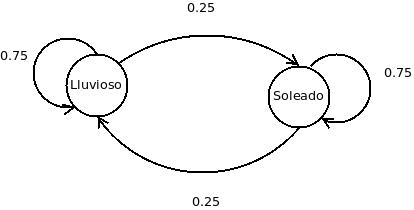
\includegraphics[width=3in]{ejemploMarkov.jpeg}
\caption{Ejemplo modelo Markov.}
\label{fig:modeloMarkov}
\end{center}
\end{figure}


\section{SSM}\label{sec:modeloSSM}

SSM o \textit{Structural Stochastic Modeling} en ingl\'es es una tecnica desarrollado por Estevez-Tapiador. A grandes rasgos, esta t\'ecnica se basa en la definición de un autómata de estados finitos estocástico capaz de evaluar la probabilidad de generación de una petición concreta. El autómata permitirá, por tanto, dada una petición, evaluar si dicha petición es legítima (corresponde al modelo) y su probabilidad. En función de la probabilidad y de un umbral se clasificaran las peticiones como normales o anormales.\cite{ssm}

Esta t\'ecnica, se basa en la teor\'ia de los modelos de Markov ya que se define un autómata de estados finitos que permite evaluar la probabilidad de generaci\'on de una petici\'on, dado un modelo previamente construido.

Por otra parte, en el presente trabajo, las peticiones que ser\'as estudiadas por dicha t\'ecnica ser\'an peticiones de tipo GET del protocolo HTTP. En concreto, de las peticiones GET el elemento a estudiar ser\'an los URIs de dichas peticiones. No obstante, se puede extender para que funcione con m\'etodos de tipo POST y HEAD. 

\begin{figure}
\begin{center}
  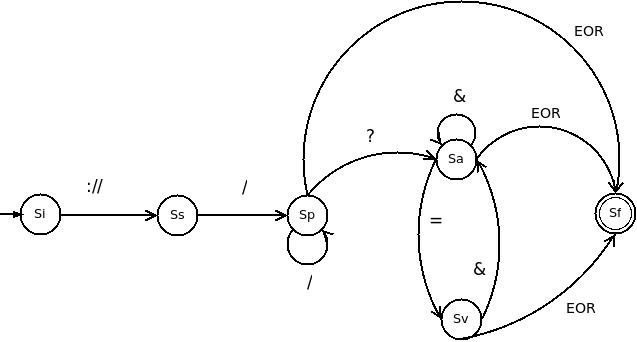
\includegraphics[width=\linewidth]{ssm.jpeg}
  \caption{Automata del modelo SSM}
  \label{fig:ssm}
\end{center}

\end{figure}

Este hecho hace que el autómata de SSM deba tomar una cierta topolog\'ia para que de esta forma se puedan reconocer los URIs de cada petici\'on. Dicha topolog\'ia se infiere a tráves de la sint\'axis de los URIs. En la figura \ref{fig:ssm} se muestra la topolog\'ia del autómata.

Las transiciones del autómata vienen dada, por las especificaciones de las sintaxis de los URIs, que est\'an descritas en el RFC 3986. Adem\'as, se puede observar en la figura \ref{fig:ssm} que el autómata tiene un estado inicial ($S_{I}$), un estado del ``host'' ($S_{S}$), un estado de segmento de ruta ($S_{P}$), un estado atributo ($S_{A}$), un estado valor ($S_{V}$), un estado final ($S_{F}$) y un estado sumidero ($S_{OOS}$) en el que se termina si el URI no es sint\'acticamente correcto.

Si una petici\'on del protocolo HTTP anexa un URI que no puede ser reconocido por el autómata descrito con anterioridad implicar\'a que el URI de dicha petici\'on no est\'a bien construido sintácticamente.

Adem\'as, existirá un vocabulario diferente para los estados $S_{S}$, $S_{P}$, $S_{A}$ y $S_{V}$. Estos vocabularios, son construidos, a partir de tomar m\'ultiples peticiones libres de ataques realizadas al servidor. 

Entonces, en resumen, lo que hace la t\'ecnica de SSM para detectar intrusiones es verificar la sintaxis del URI de las peticiones enviadas al servidor a tráves del autómata descrito con anterioridad y, al mismo tiempo, se estudia segmento por segmento del URI la probabilidad que tiene cada palabra de aparecer en un estado determinado del autómata, para as\'i verificar si el URI que viene anexado al la petici\'on es una cadena de caracteres que probabilísticamente corresponde a un petici\'on normal o no.

Teóricamente, el modelo utilizado por SSM es el siguiente \cite{tesisMexico}:

\begin{itemize}
\item Q: es el conjunto de estados ($S_{I}$,$S_{S}$,$S_{P}$,$S_{A}$,$S_{V}$,$S_{F}$,$S_{OOS}$).
\item $\theta$: es el conjunto de s\'imbolos observables que se encuentran en el vocabulario de cada estado.
\item A: es la matriz de probabilidad de transiciones entre estados
\item B: es un conjunto de vectores que contiene la probabilidad de las palabras observadas en cada estado. ($B_{I}$,$B_{S}$,$B_{P}$,$B_{A}$,$B_{V}$,$B_{F}$,$B_{OOS}$).
\item $\Pi$: es el vector de probabilidades iniciales, cuyos valores est\'an determinados por la topolog\'ia del modelo. 
\end{itemize}

\subsection*{Evaluación}
\label{subsec:exprIndice}

Dado un conjuntos de observaciones $0 = o1,o2,...,oT$. Cada una pertenecientes a los estados $Q = q1,q2,..,qT$. En principio, se puede realizar la evaluación de un URI, dado un modelo $\lambda$,  calculando la probabilidad del conjunto completo de observaciones O del modelo $\lambda$ siguiendo el patrón de la secuencia de estados Q. Es decir:

\begin{equation}
P(O|\lambda,Q) = \pi_{q1}b_{q1o1}\prod_{t=1}^{T-1}a_{q_{t}q_{t+1}}b_{q_{t+1}o_{t+1}}
\end{equation}

Para evitar problemas de desbordamiento de calcula el logaritmo de la probabilidad en lugar de la probabilidad.

\begin{equation}\label{eq:Probabilidad}
log(P(O|\lambda,Q)) = log(\pi_{q1}b_{q1o1}\prod_{t=1}^{T-1}a_{q_{t}q_{t+1}}b_{q_{t+1}o_{t+1}})
\end{equation}

Si se considera que las probabilidades iniciales son cero excepto para S1 y que las probabilidades de transición son equivalentes a 1. Entonces, se tendría que la fórmula presentada en \ref{eq:Probabilidad} se podría resumir en la siguiente:

\begin{equation}
P(O|\lambda,Q) = \sum_{t=1}^{T}b_{q_{t}o_{t}}
\end{equation}

Entonces, en primera instancia se podría decir que el índice de anormalidad de un URI U, dado un modelo $\lambda$, se puede obtener de la siguiente forma:

\begin{equation}\label{eq:Probabilidad2}
N_{s} = -log(P(U|\lambda))
\end{equation}

La fórmula \ref{eq:Probabilidad2} será aplicada sólo si el URI U llega al estado final Sf, de otra manera al índice de anormalidad Ns se le será asignado $\infty$, es decir:

\begin{equation}\label{eq:Ns1}
N_{s} = 
	\begin{cases} 
      -log(P(U|\lambda)) & $si $  q_{t} = S_{f} \\
      \infty & $si $  q_{t} \neq S_{f} \\ 
   \end{cases}
\end{equation}

Como se puede observar en la fórmula \ref{eq:Ns1}, mientras menor sea la probabilidad de aparición de las observaciones, mayor será el índice de anormalidad, por esta razón, una vez calculado el índice, se podría decir que un URI U es anómalo, si el índice de anormalidad es mayor o igual a un umbral de detección $\theta$ de lo contrario se dirá que el URI no posee anomalías, esto es:

\begin{equation}\label{eq:ClaseU}
Clase(U) = 
	\begin{cases} 
      Normal & $si $  N_{s}(U) \leq \theta \\
      Anomalo & $si $  N_{s}(U) > \theta \\ 
   \end{cases}
\end{equation}


El umbral de detección es un parámetro que se calcula de forma experimental. Durante la pruebas se busca conseguir un valor $\theta$ con el cual se pueda obtener la proporción óptima entre las detecciones de anomalías correctas y los falsos positivos. 

No obstante, la fórmula presentada en el apartado \ref{eq:Ns1} posee algunos inconvenientes ya que no se estipula el caso en el que existan problemas de entrenamiento insuficiente que será presentado en la sección o que los diferentes vectores B, tengan diferente número de observaciones. El segundo caso provoca un inconveniente a la hora de realizar la evaluación ya que el acumulado de las probabilidades de los vectores B estarán ligados a la longitud de los mismos. Para solucionar dicho problema se utilizara la propuesta de Estévez [Estévez-Tapiador 2004a], en el que se establece como factor de compensación la probabilidad de observación para de esta manera obtener una probabilidad normalizada. Esta sería la siguiente expresión:

\begin{equation}\label{eq:sumB}
\varepsilon_{0} = E[B] = \frac{1}{M}\sum_{i=1}^{M}b_{i}
\end{equation}

Por otra parte, el entrenamiento insuficiente es un problema que se presenta cuando se toma una palabra durante la evaluación que no pertenezca al conjunto de palabras observadas durante el entrenamiento en el modelo. Esto puede ser debido a que la palabra es una palabra anómala o que no se entrenó lo suficiente al sistema. En este caso, la solución que se le aplicará a dicho problema será la de asignar un valor fijo de probabilidad muy baja a estos casos ( poov($S_{i}$): probabilidad fuera de vocabulario). Cada uno de los estados del modelo poseerá valores independientes de probabilidades que serán utilizados una vez se detecte este problema.

El otro caso en el que se utilizarán los valores de poov($S_{i}$), es cuando la probabilidad de una palabra que está en el vocabulario es inferior al poov($S_{i}$), es decir:


\begin{equation}\label{eq:Pqtot}
p_{qtot} = 
	\begin{cases} 
      b_{qtot} & $si $  o_{t} \in O $ y $ b_{qtot} > p_{oov}(q_{t})\\
      p_{oov} & $en otro caso$ \\ 
   \end{cases}
\end{equation}


Entonces, la nueva expresión del índice de anormalidad que toma en cuenta todas las consideraciones nombradas con anterioridad, es la siguiente:

\begin{equation}\label{eq:Ns}
N_{s} = 
	\begin{cases} 
      -Tlog(\varepsilon_{0})\sum_{t=1}^{T}log(p_{qtot}) & $si $  q_{t} = S_{f} \\
      \infty & $si $  q_{t} \neq S_{f} \\ 
   \end{cases}
\end{equation}

\subsection*{Entrenamiento}

Dada una secuencia de observaciones 0 = o1,o2,...,oT ,y  su correspondiente secuencia de estados, Q = q1,q2,...,qT.

El entrenamiento requiere de un conjunto considerable de observaciones  junto con los estados asociados a cada una de ellas.

Por lo tanto, se considerara un conjunto de entrenamiento $\omega$ de L pares de secuencias de estados

\begin{equation}
\omega = {(O^{1},Q^{1}),(O^{2},Q^{2}),...,(O^{L},Q^{L})}
\end{equation}

tal que:

\begin{equation}
\begin{aligned}
O^{i} = {o_{1}^{i},o_{1}^{i},...,o_{Ti}^{i}} \\
Q^{i} = {q_{1}^{i},q_{2}^{i},...,q_{Ti}^{i}}
\end{aligned}
\end{equation}

Entonces, para crear el vocabulario del modelo de normalidad solo se tendrá que hacer un recuento de las frecuencias de aparición relativas de los símbolos y los estados, es decir:

\begin{equation}
\theta_{Sk} = \bigcup\limits_{i=1}^{L} {o_{j}^{i}|q_{j}^{i} = S_{k}}
\end{equation}

Por otra parte, para calcular la probabilidades de observación se utilizaría la siguiente expresión:

\begin{equation}\label{eq:entrenamiento}
b_{ij} = \frac{\sum_{s=1}^{L}\sum_{t=1}^{Ts}\delta(o_{t}^{s} = v_{i,j} ,q_{t}^{s} = s_{i} )}{\sum_{s=1}^{L}\sum_{t=1}^{Ts}\delta(q_{t}^{s} = s_{i}) }
\end{equation}

Donde, $\delta$ es una función que retorna 1 si todos sus argumentos son verdaderos y 0 cuando son falsos.

\subsection*{Normalización de los URIs}
\label{sec:normalizacion}

La normalización consiste en tomar el URL en el formato en el que viene y codificarlo al formato de tipo UTF-8. Este paso evitará considerar palabras o frases iguales que estén escritas en formatos diferente como elementos distintos. 

Un ejemplo sencillo de lo que se haría en la normalización del sistema sería el siguiente:

Supongamos que al servidor de tipo HTTP recibe dos peticiones de tipo GET con los siguientes URIs:

\begin{itemize}
\item https://192.168.0.23?q=security+network
\item https://192.168.0.23?q=security\%20network
\end{itemize}
Ambos URIs poseen la misma información, sin embargo, el espacio en blanco esta codificado de manera diferente en ambos casos. Si no se lleva a cabo la normalización, la palabra "security+network" y "security\%20network" serían tomadas como dos palabras totalmente diferentes por el sistema. En este caso, la función de normalización se encargaría de traducir el primer URI al formato UTF-8 para que no exista este problema. Por lo tanto,la frase "security+network" pasaría a ser  "security\%20network".


\subsection*{Segmentación de los URIs}
\label{sec:delimitadores}

La idea de la segmentación de URI es considerar una serie de delimitadores, que delimitan áreas especificas dentro del URI.

Los delimitadores que se tomarán en cuenta para segmentar serán los asociados al estándar del protocolo HTTP. Estos son los siguientes:

\begin{itemize}
\item D1 = ://, delimitador de protocolo.
\item D2 = /, delimitador de recursos.
\item D3 = ?, delimitador de parámetros.
\item D4 = =, delimitador de asignación de atributos.
\item D5 = \&, delimitador entre parametros.
\item D6 = ASCII 32, delimitador de fin de recurso
\end{itemize}

A modo ilustrativo, se utilizará un ejemplo concreto con un URI para mostrar como funciona la segmentación en el sistema.

Supongamos que tenemos el siguiente URI:

http://159.90.9.166/consulta/?manifestacion=Pinturas+Rupestres

Entonces, la función que se encarga de segmentar tomará dicho URI y lo segmentará en las siguientes partes:

\begin{itemize}
\item http : Segmento correspondiente al protocolo del URI. 
\item 159.90.9.166 : Segmento correspondiente al ``host'' del URI. 
\item consulta : Segmento correspondiente al recursos del URI.
\item manifestacion : Segmento correspondiente al atributo del query.
\item Pinturas\%20Rupestres : Segmento correspondiente al valor del query.  
\end{itemize}

















 




\chapter{Marco técnologico}
\label{capituloTecnologico}

\section{Herramientas utilizadas}

\subsection{Bro}

Bro es un software ``open source'' cap\'az de analizar a detalle las actividades que ocurren en la red. Se utiliza principalmente para inspeccionar todo el tráfico y detectar signos de actividad sospechosa. Sin embargo, Bro soporta una amplia gama de tareas de análisis de tráfico incluso fuera del dominio de seguridad, incluyendo mediciones de rendimiento y ``trouble-shouting''.\cite{Bro}

Este software, posee un conjunto extenso de $"logs"$ que registran las actividades que se observan en la red. Estos $"logs"$ almacenan información de la capa de aplicación, como por ejemplo, los URIs y las respuestas del servidor en una sesión de tipo HTTP, o las solicitudes y respuestas DNS en una sesión DNS. Bro escribe todos estos datos en archivos con formatos bien predeterminados con la intención de facilitar el procesamiento de la información almacenada por programas externos. No obstante, el usuario tiene la posibilidad de elegir el formato en el que se almacenan los datos.

Por otra parte, Bro incluye también un lenguaje de $"scripting"$, Turing completo y orientado a eventos, cuya funci\'on es extender y personalizar las funcionalidades primarias que otorga el mismo. Este lenguaje de $"scripting"$ posee una biblioteca estándar. 

Así mismo, el lenguaje de Bro posee diversos ``frameworks'' que facilitan el trabajo al momento de programar nuevas funcionalidades. Los ``frameworks'' utilizados en el sistema implementado fueron: el ``Input Framework'' y el ``Logging Framework''.
El ``Input Framework'' permite leer de manera mas cómoda y eficiente la información que se encuentra dentro de los $"logs"$ del sistema.
Este $"framework"$ posee dos modalidades. La primera modalidad consiste en leer la información que se encuentra dentro de los $"logs"$ para luego almacenarla en una estructura de datos de tipo $"table"$. La segunda modalidad lee la información y la envía a un evento anteriormente programado.
Por otra parte, el ``Logging Framework'', tiene como tarea facilitar el manejo y la escritura de los $"logs"$. Este, permite crear, escribir datos de forma organizada y filtrar información de los $"logs"$.

Como se mencionó con anterioridad, el lenguaje de $"scripting"$ de Bro es un lenguaje orientado a objetos. Sin embargo, es importante recalcar, que el núcleo o motor principal de Bro es el motor de eventos, el cual reduce la información entrante de la red, en eventos de alto nivel. Por ejemplo, si se recibe una solicitud de tipo HTTP, Bro se encargará de convertir la misma en un evento de tipo $"http\_request"$ en donde se almacenará información como: la dirección IP, los puertos involucrados, el URI y la versión de tipo HTTP en uso.

A su vez, los eventos creados por Bro a partir de la información entrante de la red son enviados a los manejadores de eventos escritos en el lenguaje de $"scripting"$ de Bro. Estos manejadores administran dichos eventos a tráves de una cola ordenada.

En Bro hay eventos primitivos, como es el caso de $"http\_request"$ --evento generado por las solicitudes tipo HTTP -- , $"dns\_request"$, --evento generado por las solicitudes tipo DNS-- , $"bro\_init"$ -- evento generado al momento en el que Bro inicializa-- y $"bro\_done"$ --evento que se genera cuando se culminan de realizar todas las tareas que se deben realizar--. Sin embargo, este software brinda la capacidad a los programadores de implementar eventos propios. Estos eventos son un tipo especial de función que poseen las características de: no retornar valores, poder ser programados para una ejecución posterior y poseer una prioridad asociada y configurable que determine el orden en el que serán ejecutados.

Un ejemplo de la implementación de un evento en el lenguaje de Bro sería la siguiente:

\begin{verbatim}
event myevent(s: string)
	{
	print "myevent", s, n;
	}
\end{verbatim}

Así como se pueden escribir eventos en Bro, también se pueden implementar funciones haciendo uso de la palabra reservada $"function"$. Una función en Bro luciría de la siguiente manera":

\begin{verbatim}

function factorial(n: count): count
    {
    if ( n == 0 )
        return 1;
    else
        return ( n * factorial(n - 1) );
    }

\end{verbatim}

Por otra parte, el lenguaje de Bro además de permitir implementar eventos y funciones, posee diversos tipos y estructura de datos que facilitan el manejo de la información. 
El conjunto de tipos de datos que posee el mismo se basa en los tipos de datos comunes que encontramos en la mayoría de los lenguajes de programación como: el $"int"$, que representa los números enteros de 64 bits, $"double"$ que representa los números flotantes de 64 bits, $"bool"$ para los booleanos y $"count"$  para los números enteros sin signo de 64 bits, y en un grupo de tipos de datos  mas especifico como: el $"addr"$ que representa direcciones ip, $"port"$ para los puertos de la capa de transporte, $"subnet"$ para las mascaras de subred, $"time"$ para almacenar datos que representen tiempo, $"interval"$ para representar intervalos de tiempo y $"pattern"$ para las expresiones regulares.

Las estructura de datos que permite el lenguaje son: los conjuntos ("set"), las tablas ("table"), vectores ("vector") y registros ("record").

\subsection{GitHub}

\subsection{Wireshark}

\section{Estación de trabajo}
\chapter{Marco Metodológico}
\label{capituloMetodologico}

En este capítulo, se explicara la metodología de trabajo que se utilizo en cada una de las fases del proyecto. 

La realización del sistema, estuvo dividida en dos grandes fases: la primera fase, consistió en hacer investigaciones y estudiar las herramientas a utilizar y la segunda fase estuvo centrada en el diseño, la implementación y la ejecución de las pruebas correspondientes al  sistema. Ambas fases fueron tratadas con metodologías diferentes que serán explicadas a continuación.

\section{Explicación de la Metodología Aplicada}


El proyecto estuvo conformado por varias etapas. En primer lugar,se realizó un estudio sobre los IDS y sus tipos; el sistema SSM, los URI y el protocolo HTTP. Luego, se hizo un análisis de la herramienta Bro, para después diseñar la arquitectura del sistema, realizar la implementación del mismo y hacer las pruebas correspondientes.

Para trabajar las dos primeras fases del proyecto realizado, se estableció un periodo de tiempo para cada una de las misma en una reunión establecida con el tutor industrial.
Entre cada uno de los periodos establecidos en cada fase, existían reuniones con el tutor para solventar las dudas teóricas que iban surgiendo a medida que se realizaban las investigaciones.

El resto de las etapas fue abordada mediante una metodología ágil. Este tipo de métodos,  promueven el desarrollo del software de manera iterativa en donde el ciclo de diseñar, codificar y realizar pruebas se repita de manera continua durante el proceso de desarrollo del software. El uso de este tipo de metodología incrementa el ciclo de vida de los productos\cite{agil}.

La organización de la segunda fase del proyecto consistió ir desarrollando cada uno de los módulos del sistema de manera iterativa, es decir, se diseñaba la arquitectura de uno de los módulos, se implementaban las funcionalidades, se realizaban las pruebas funcionales y luego se iniciaba la otra iteración con el próximo módulo. Al inicio de cada una de las iteraciones, se realizaba una reunión en donde se plantean las tareas que se debían realizar, junto con el tiempo estimado que tomarían las mismas. En dicha reunión se discutían, se ajustaban y si era necesario se agregan tareas a la lista.  Durante el transcurso de las  iteraciones se pautaron reuniones cada dos semanas en donde se mostraba el producto al tutor industrial y se planteaban las dudas que habían surgido durante el desarrollo del proyecto.

Cuando se culminaba de desarrollar la arquitectura, implementar y probar la funcionalidad de un módulo se planificaban las tareas del próxima iteración, y se volvía a realizar un reunión para ajustar las mismas. Este procedimiento se llevó a cabo con los tres módulos que conforman el sistema, es decir, el desarrollo del proyecto, estuvo conformado por tres iteraciones. 
Luego de  finalizar las tres iteraciones para desarrollar los tres módulos que conforman el sistema, se procedió a realizar pruebas operativas sobre el mismo.

El proyecto estuvo conformado por varias etapas. En primer lugar,se realizó un estudio sobre los IDS y sus tipos; el sistema SSM, los URI y el protocolo HTTP. Luego, se hizo un análisis de la herramienta Bro, para después diseñar la arquitectura del sistema, realizar la implementación del mismo y hacer las pruebas correspondientes.

Para trabajar las dos primeras fases del proyecto realizado, se estableció un periodo de tiempo para cada una de las misma en una reunión establecida con el tutor industrial.
Entre cada uno de los periodos establecidos en cada fase, existían reuniones con el tutor para solventar las dudas teóricas que iban surgiendo a medida que se realizaban las investigaciones.

El resto de las etapas fue abordada mediante una metodología ágil. Este tipo de métodos,  promueven el desarrollo del software de manera iterativa en donde el ciclo de diseñar, codificar y realizar pruebas se repita de manera continua durante el proceso de desarrollo del software. El uso de este tipo de metodología incrementa el ciclo de vida de los productos.

La organización de la segunda fase del proyecto consistió ir desarrollando cada uno de los módulos del sistema de manera iterativa, es decir, se diseñaba la arquitectura de uno de los módulos, se implementaban las funcionalidades, se realizaban las pruebas funcionales y luego se iniciaba la otra iteración con el próximo módulo. Al inicio de cada una de las iteraciones, se realizaba una reunión en donde se plantean las tareas que se debían realizar, junto con el tiempo estimado que tomarían las mismas. En dicha reunión se discutían, se ajustaban y si era necesario se agregan tareas a la lista.  Durante el transcurso de las  iteraciones se pautaron reuniones cada dos semanas en donde se mostraba el producto al tutor industrial y se planteaban las dudas que habían surgido durante el desarrollo del proyecto.

Cuando se culminaba de desarrollar la arquitectura, implementar y probar la funcionalidad de un módulo se planificaban las tareas del próxima iteración, y se volvía a realizar un reunión para ajustar las mismas. Este procedimiento se llevó a cabo con los tres módulos que conforman el sistema, es decir, el desarrollo del proyecto, estuvo conformado por tres iteraciones. 
Luego de  finalizar las tres iteraciones para desarrollar los tres módulos que conforman el sistema, se procedió a realizar pruebas operativas sobre el mismo.

\chapter{Desarrollo de Pasantías}
\label{capitulo3}
\lhead{Capítulo 3. \emph{Diseño del sistema}}

\section{Estado del Arte}

En esta etapa del proyecto se realizó una investigación sobre los conceptos fundamentales del sistema a implementar. Las definiciones estudiadas fueron: el protocolo HTTP, los URIs, detector de intrusiones (IDS), modelo de Markov y SSM.
El resumen de esta investigación se encuentra en el capítulo \ref{capitulo2} del presente trabajo.

\section{Análisis de Bro}

En esta etapa del proyecto se descargó, se instaló y se estudio la herramienta Bro y su lenguaje de ``scripting''. Bro, es la herramienta principal que se utilizó en la implementación del sistema. Un resumen de esta y de su lenguaje de programación se encuentra en la sección \ref{ssec:Bro}.

\section{Diseño de la arquitectura del sistema}

Esta sección tiene la intención de mostrar la visión general del modelado del sistema que se realizó a partir de las bases teóricas. Aquí, se explicará la arquitectura, el diseño y el modo en el que el IDS basado en SSM interactuará con Bro. Además, se detallaran las salidas y los datos de configuración
que va a considerar el sistema para su correcto funcionamiento.

\subsection{Arquitectura del sistema}

La arquitectura del detector de intrusiones que se muestra en el presente trabajo se basa en una arquitectura modular la cual está conformada por tres modulo. Un modulo para realizar la segmentación de los URIs, otro  para realizar la evaluación y un tercero para realizar el entrenamiento.

A grandes rasgos, el módulo de segmentación, se encargará de tomar los URIs previamente filtrados de las solicitudes de tipo HTTP/GET, lo normalizará y lo segmentará de la forma en la que se explicó en el apartado de ``segmentación'' de la sección \ref{sec:delimitadores}.

Por otra parte, el modulo de evaluación se encargará de evaluar la probabilidad de generación de cada uno de los segmentos del URI generados por el módulo de segmentación para al final decidir si el URI de la solicitud enviada al servidor web es anómalo o no.

Por último, el modulo de entrenamiento será el encargado de crear el modelo de normalidad del sistema. Para esto, el sistema recibirá solicitudes libres de ataques e irá calculando la probabilidad de aparición de cada una de las palabras que aparecen en las mismas.

Tanto el modulo de evaluación, como el modulo de entrenamiento son dependientes del modulo de segmentación ya que requieren de los segmentos de URI generados por eso para realizar su trabajo. 

La arquitectura del sistema queda detallada en la figura \ref{fig:arquitectura}.

\begin{figure}[!htb]
\begin{center}
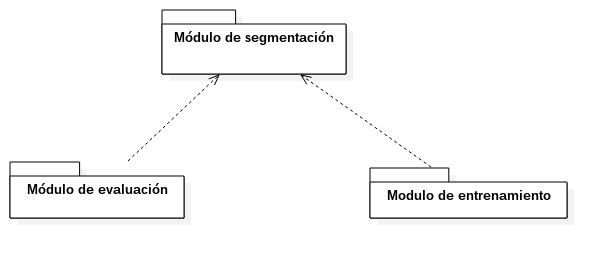
\includegraphics[width=3in]{./img/arquitectura.png}
\caption{Arquitectura del sistema.}
\label{fig:arquitectura}
\end{center}
\end{figure}


Así mismo, es importante mencionar que el sistema contará con varios modos de operación que serán explicados a continuación:

\begin{itemize}
\item Modo evaluación: En este modo de operación solo se activarán los módulos de segmentación y evaluación del sistema. A manera general, esta modalidad, se encargará de recibir los URI previamente extraídos de las peticiones de tipo HTTP/GET, segmentarlos a tráves del módulo de segmentación, para luego evaluar si el mismo es anómalo o no
haciendo uso del módulo de evaluación. El funcionamiento de esta modalidad queda detallado en la figura \ref{fig:modoSistema}.
\item Modo entrenamiento ``Online'': En este modo de operación solo trabajaran los módulos de segmentación y entrenamiento. En esta modalidad el módulo de entrenamiento tomará los segmentos arrojados por el módulo de segmentación, calculará la probabilidad de aparición de los mismos para de esta manera ir modificando un modelo de normalidad previamente establecido. El funcionamiento de esta modalidad queda
detallado en la figura \ref{fig:modoSistema}.
\item Modo entrenamiento ``Offline'': Esta modalidad del sistema en análoga al modo de entrenamiento ``Online''. El único aspecto que diferencia a ambas modalidades es que cuando el sistema funciona en modo ``Offline'' no se toma en cuenta, ni se modifica un modelo de normalidad previamente construido. La salida de este modo de entrenamiento sera un modelo de normalidad construido desde cero.El funcionamiento de esta modalidad queda detallado en la figura \ref{fig:modoSistema}.
\end{itemize}

\begin{figure}[!htb]
\begin{center}
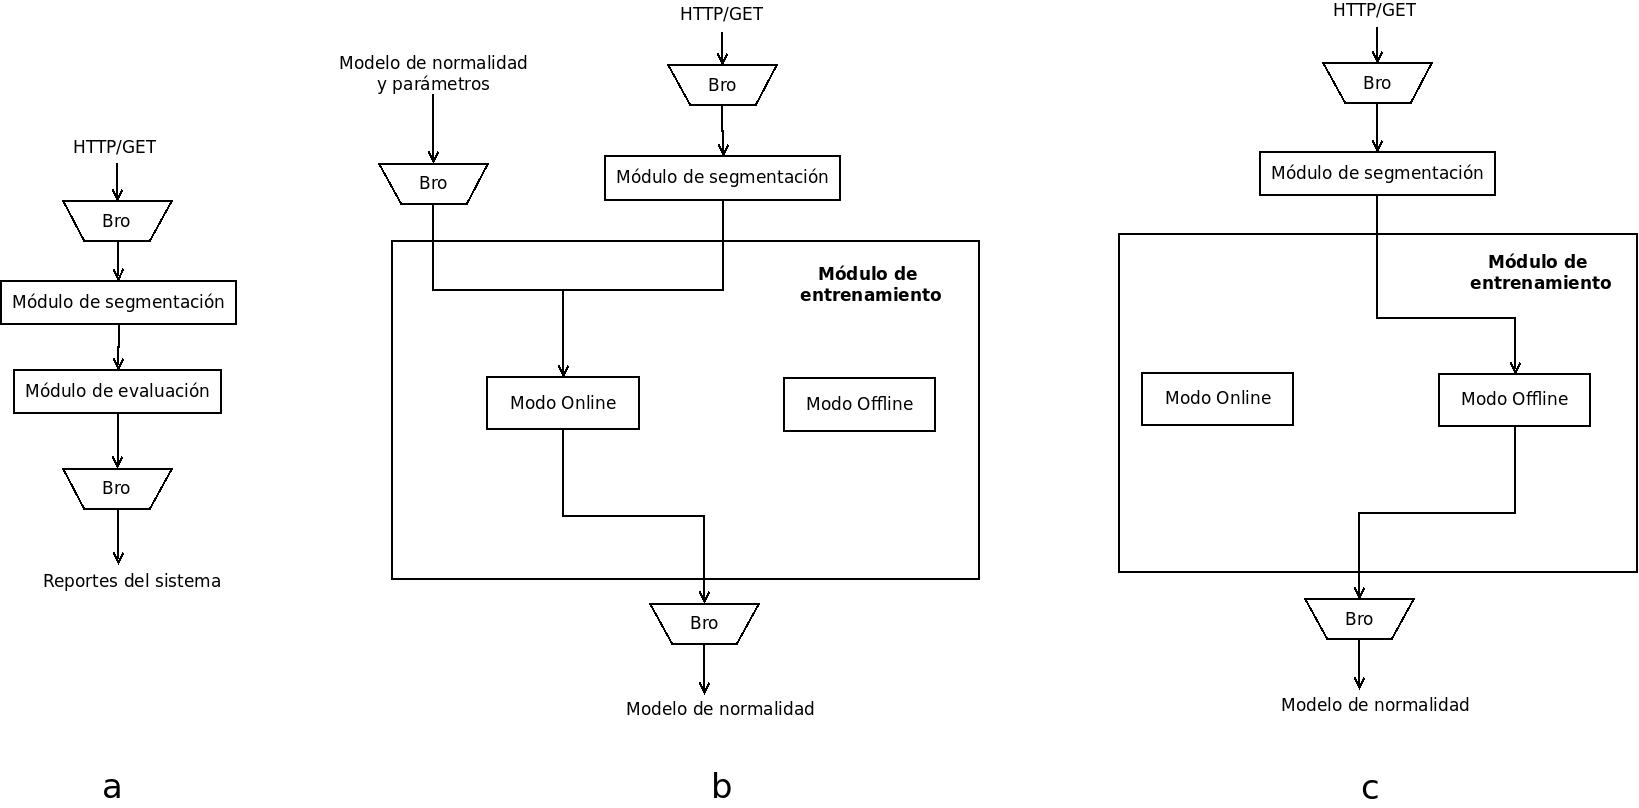
\includegraphics[width=\linewidth]{./img/modoOperacion.jpeg}
\caption{Modo evaluación (a), modo entrenamiento ``Online'' (b), modo entrenamiento ``Offline'' (c).}
\label{fig:modoSistema}
\end{center}
\end{figure}


\subsection{Filtrado de paquetes HTTP/GET}

Esta funcionalidad se encargará de observar los paquetes de la red y filtrar aquellos de tipo HTTP/GET. Una vez obtenido este tipo de paquetes, esta función extraerá el URI adjunto al mismo.

\subsection{Módulos}

En esta sección se describirán las tareas de cada uno de los módulos que conformar la arquitectura detallada en la figura \ref{fig:arquitectura}, el modo en el que se subdividieron dichas tareas, los datos de entrada y salida, y la interacción que existe entre los mismos.

\subsubsection{Módulo de segmentación}

El modulo de segmentación es un elemento clave dentro de la construcción del IDS basado en SSM, es por eso que su buen diseño e implementación es importante para el buen funcionamiento del sistema. Este se encarga, como se mencionó anteriormente,de tomar el URI que proviene de la solicitud de tipo HTTP/GET que se le hace al servidor HTTP capturado por Bro, normalizarlo y segmentarlo siguiendo las especificaciones que se explicaron en la sección \ref{sec:delimitadores}. 

Es evidente entonces, que este modulo consta de dos funcionalidades fundamentales: la normalización de los URIs y la segmentación.  La normalización se encargará de tomar el URI de las peticiones HTTP/GET entrantes y codificarlo a formato UTF-8. Normalizar es un paso importante dentro del sistema  ya que se estandarizar la forma en las que están escritos los URIs facilita tanto la evaluación como el entrenamiento en el sistema. Por otra parte, la salida arrojada por esta función de normalización será tomada por la de segmentación, quien a su vez se encargará de segmentar el URI de la forma en la que se explica en la sección \ref{sec:delimitadores}, es decir, el URI se dividirá en las diferentes partes estipuladas en el RFC 3986: el ``host'', la ruta, los argumentos, los valores y el ``fragment''.

 En las base teórica, la segmentación de los URIs se realiza mediante un autómata que se encarga de reconocer (realizar un análisis sintáctico) y evaluar en cada uno de sus estados la probabilidad de generación de cada uno de los segmentos.  No obstante, en la función de segmentación del sistema implementado, esta tarea se modeló mediante un analizador sintáctico que hace uso de una gramática (libre de contexto) de atributos que genera el mismo lenguaje que reconoce el autómata presentado en la figura ~\ref{fig:automata}, es decir, el lenguaje de los URI.

En la figura \ref{fig:arquiSegmentacion} se puede apreciar el diagrama de bloques que refleja el funcionamiento del módulo de segmentación.

\begin{figure}[!htb]
\begin{center}
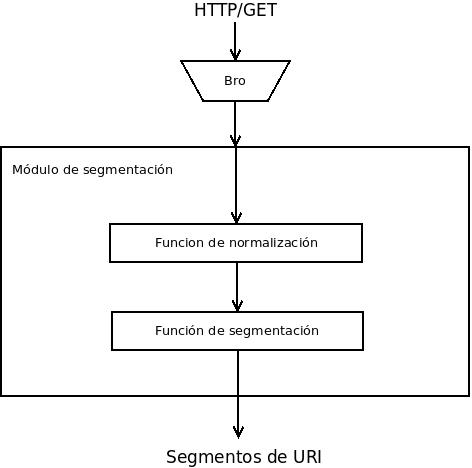
\includegraphics[width=3in]{./img/segArquiCompleta.jpeg}
\caption{Diagrama de bloques del módulo de segmentación.}
\label{fig:arquiSegmentacion}
\end{center}
\end{figure}

\subsubsection{Módulo de evaluación}
\label{sec:evaluacion}

El módulo de evaluación, es el encargado de evaluar la probabilidad de generación de cada uno de los segmentos del URI otorgados por el modulo de segmentación, dado un modelo de normalidad. Una vez calculadas estas probabilidades, el modulo se encargará de calcular un índice de anormalidad del URI mediante el uso de las formulas descritas en la sección ~\ref{subsec:exprIndice} para luego compararlo con un parámetro $\theta$ (\ref{eq:ClaseU}) y de este modo saber si los segmentos de URI que ingresaron como entrada posee alguna anormalidad o no. Luego de realizar esta evaluación, el modulo se encargara de escribir los reportes del sistema en un ``log''.

El módulo de evaluación, está conformado por dos grandes funcionalidades: una que se encargará de leer el modelo de normalidad y  otra que calculará el índice de anormalidad y evaluará si el mismo es anómalo o no. 

El modelo teórico que fue explicado en la sección ~\ref{sec:modeloSSM} posee elementos como: un conjunto ``S'' de estados, un conjunto ``O'' de símbolos observables que se encuentran en cada estado, una matriz ``A'' que contiene la probabilidad de transición entre estados, un conjunto ``B'' de vectores que contiene la probabilidad de las palabras observadas en cada estado y un vector de probabilidades iniciales. No obstante, los únicos elementos del modelo que se necesitan ingresar en el sistema para que este funcione y realice las tareas de evaluación son: el conjunto ``O'' de símbolos observables que se encuentra en cada estado y el conjunto de vectores ``B''. El conjunto ``B'' es necesario para resolver la expresión \ref{eq:sumB}. Por otra parte, es necesario hacer uso tanto de ``B'' como ``O'' para obtener el valor de $b_{qtot}$ presentado en la ecuación \ref{eq:Pqtot}. Este elemento es sumamente importante para calcular el índice de anormalidad. Por otra parte, será necesario introducir al sistema los valores de probabilidad de fuera de vocabulario (Poov), ya que son necesarios para obtener el valor de $p_{qtot}$, presente en la ecuación \ref{eq:Pqtot}, en caso que una cadena de caracteres del URI que se esté analizando no se encuentre en el conjunto de observaciones ``O''. Además, se requiere el valor del parámetro $\theta$ para evaluar el índice de anormalidad según lo estipulado en la ecuación \ref{eq:ClaseU} .

    Entonces, en conclusión, los parámetros que requieren ser introducidos al sistema de detección de intrusiones para que este funcione de manera correcta son: el conjunto de observaciones de cada estado (O), el conjunto de vectores de probabilidad de las palabras observadas en cada estado ( $B_{S}, B_{P}, B_{A}, B_{V}$ ), los valores de probabilidad de fuera de vocabulario, es decir $P_{oovS}, P_{oovP}, P_{oovA}, P_{oovV}$ y el valor del parámetro $\theta$. Todos estos parámetros serán leídos por la función de lectura del modulo de evaluación.
    
Una vez leídos los parámetros necesarios para que el sistema funcione, estos serán enviados a la función de evaluación junto a los segmentos de URI dados por el módulo de segmentación. Una vez recibidos los datos de entrada, esta función se encargará de hallar el índice de anormalidad ($N_{s}$) mediante la expresión \ref{eq:Ns} para, de este modo compararlo con el parámetro $\theta$ como se indica en \ref{eq:ClaseU}.No obstante, las tareas de calculo y evaluación del índice de anormalidad, fueron subdivididas a su vez, en cuatro funciones. La primera de las funciones será la encargada de calcular tanto el $\varepsilon_{0}$ que aparece en la expresión \ref{eq:sumB} como la sumatoria de los logaritmos de los $p_{qtot}$ que se encuentra en \ref{eq:Ns}; la segunda función tomará el valor de $\varepsilon_{0}$ y la sumatoria de los logaritmos de los $p_{qtot}$ que calculó la primera función y procederá a efectuar todas las operaciones que hay en la expresión \ref{eq:Ns} para de este modo obtener el índice de anormalidad, $N_{s}$; por otra parte, la tercera función tendrá como tarea comparar el índice de anormalidad $N_{s}$ calculado por la tercera función, con el parámetro $\theta$ como se indica en \ref{eq:ClaseU}; la cuarta será la encargada de escribir en un archivo de texto aquellos URIs anómalos.

El diagrama de bloques presente en la figura \ref{fig:arquiEvaluacion} representa el funcionamiento del módulo de evaluación.

\begin{figure}[!htb]
\begin{center}
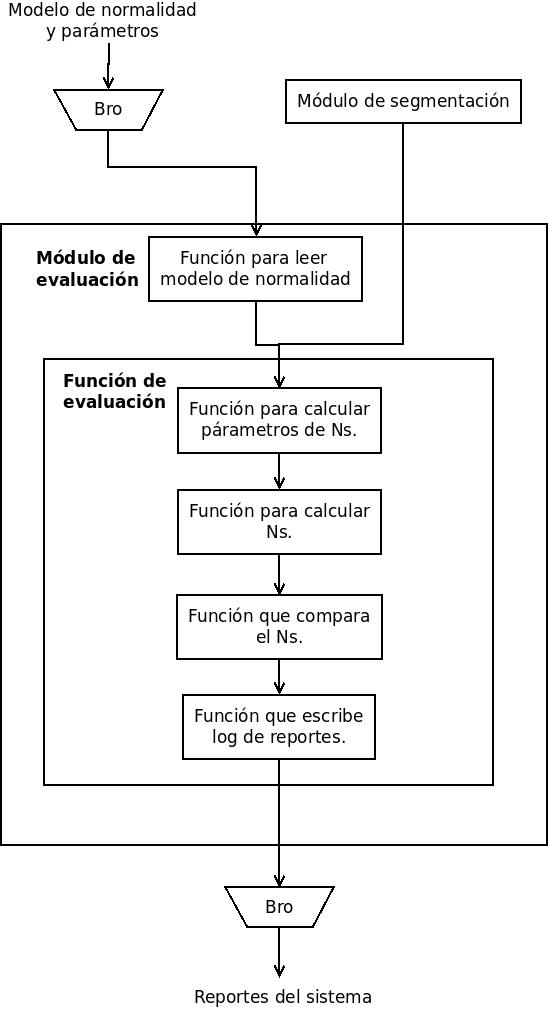
\includegraphics[width=3in]{./img/evalArqui.jpeg}
\caption{Diagrama de bloques del módulo de evaluación.}
\label{fig:arquiEvaluacion}
\end{center}
\end{figure}

\subsubsection{Módulo de entrenamiento}\label{sec:entrenamiento}

El modelo de normalidad es uno de los aspecto importantes dentro del IDS basado en SSM ya que a partir de la información que este almacena se podrá decidir si un URI es anómalo o no dependiendo de la similitud que posea este con los datos que almacena el modelo. Por esta razón, realizar un modelo de normalidad apropiado es un aspecto  importante para que el módulo de evaluación haga detecciones de intrusiones más certeras.

El módulo encargado de elaborar los modelos de normalidad será el módulo de entrenamiento. A grandes rasgos, este se encargará de recibir un conjunto de segmentos libres de ataques proporcionados por el módulo de segmentación para ir calculando la probabilidad de aparición de cada una de las palabras que aparecen en los mismos, para finalmente, escribir en un archivo toda la información recolectada, es decir, el conjunto de palabras observadas mientras se hacía el entrenamiento, sus probabilidades de aparición y el estado del autómata en el que se observaron las mismas.

Este módulo consta de dos modos: el modo ``Offline'' y el modo ``Online''. La  diferencia fundamental entre el modo ``Online'' y el ``Offline'' es que en el primero necesita como entrada un modelo de normalidad ya construido y los segmentos de URI proporcionados por el módulo de segmentación. Una vez realizado el entrenamiento, esta modalidad se encargará de actualizar el modelo que se leyó al inicio. Por otra parte, el modo ``Online'' solo requiere como entrada los segmentos de URI y como salida proporcionará un  modelo de normalidad construido desde cero.

El modo de entrenamiento ``Offline'' fue dividido en tres funciones. La primera función irá observando los segmentos de los URIs de las peticiones que van llegando y contará el numero de veces que cada segmento fue observado durante el entrenamiento. La segunda función, toma el resultado de las observaciones realizadas por la primera función y calculará la probabilidad de aparición de cada uno de los segmentos haciendo uso de la formula \ref{eq:entrenamiento}. La tercera función tomara los resultados otorgados por la segunda función y los escribirá en un archivo de texto. Este archivo representara el modelo de normalidad construido.

Por otra parte, las tareas a realizar por el modo de entrenamiento ``Online'' fueron divididas de igual modo en tres funciones: La primera función se encargara de leer el modelo de normalidad; la segunda se encargará de tomar el modelo de normalidad leído por la primera función y el conjunto de segmentos de URI del módulo de segmentación. Esta información sera utilizada por la misma para ir calculando la probabilidad de aparición de los segmentos observados. La tercera función se encargara de recibir los resultados obtenidos por la segunda función y actualizara el modelo de normalidad previamente existente.

En la figura \ref{fig:arquiEntrenamiento} se puede apreciar el diagrama de bloques que describe el funcionamiento del módulo de entrenamiento.

\begin{figure}[!htb]
\begin{center}
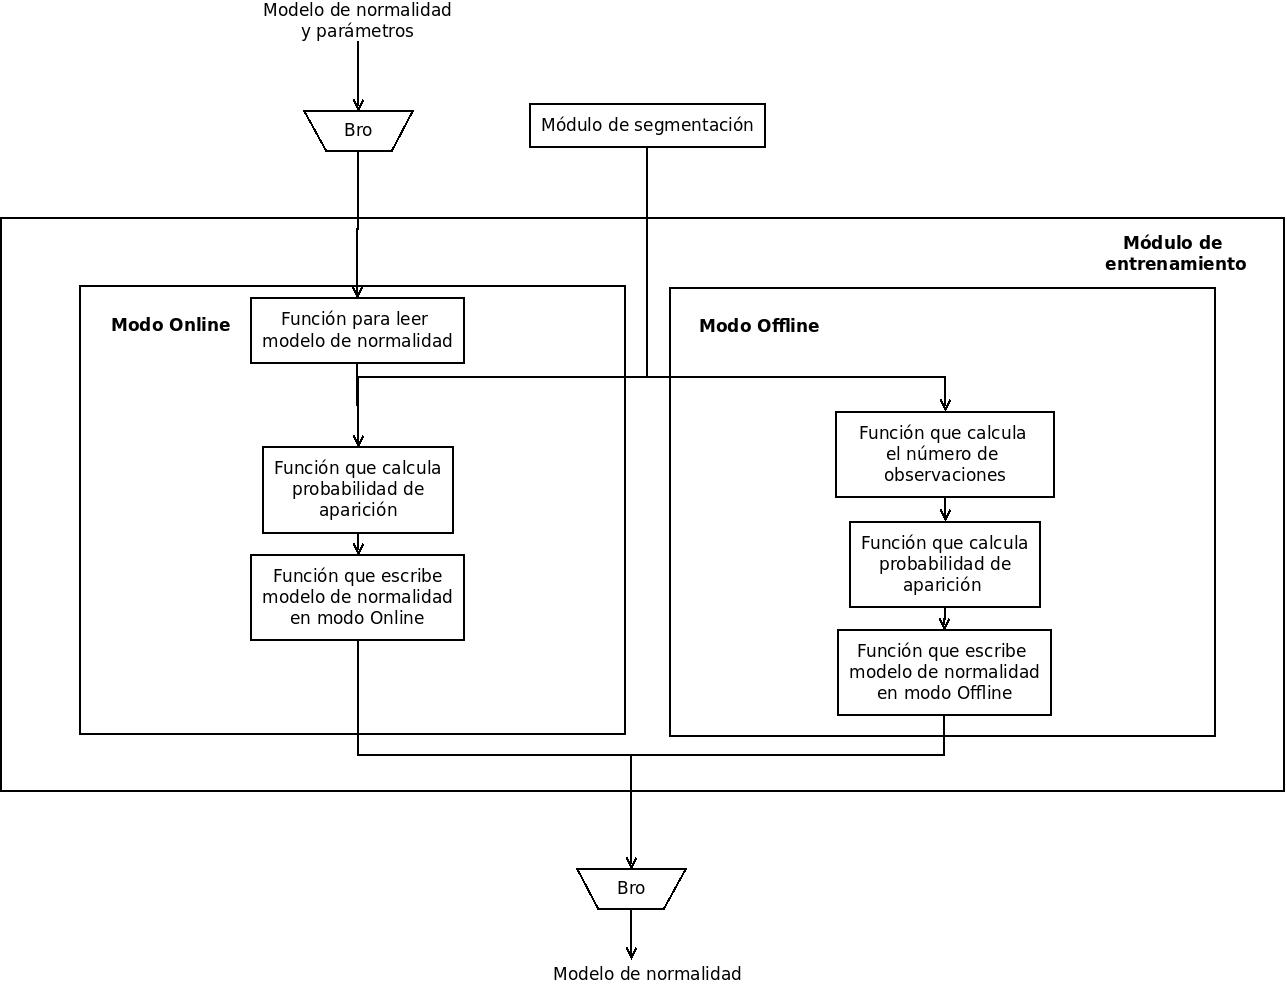
\includegraphics[width=3in]{./img/entrenamArqui.jpeg}
\caption{Diagrama de bloques del módulo de entrenamiento.}
\label{fig:arquiEntrenamiento}
\end{center}
\end{figure}

\section{Implementación del Sistema}

Una vez descrita la arquitectura modular del sistema y las funcionalidades asociadas a los diferentes componentes del sistema, en este capítulo se detallarán las cuestiones más relevantes en cuanto a su implementación.
Así, en primer lugar, se describirán como se implementó el filtro de paquetes HTTP/GET, para luego explicar las estructuras de datos utilizadas por cada uno de los módulos; los parámetros de entrada, salida y la implementación de las funciones que los componen.

\subsection{Filtrado de Paquetes HTTP/GET}

El módulo de segmentación requiere como entrada los URIs extraídos de las peticiones de tipo HTTP/GET. Esta tarea se realizó haciendo uso de las herramientas brindadas por Bro. En concreto, esta funcionalidad fué implementada con un evento primitivo de Bro llamado ``http request''. Este evento se genera y almacena la información de paquetes HTTP cuando son percibidos por dicha herramienta en la red. Su formato es el siguiente:

\textbf{http request}(c: \textbf{connection}, method: \textbf{string}, original\_URI: \textbf{string},
unescaped\_URI: \textbf{string}, version: \textbf{string})
donde:
\begin{itemize}
\item c: es una estructura de datos de tipo ``connection'' que almacena de manera desglosada la información del mensaje HTTP.
\item method: Es el método extraído de la petición (e.g., GET,POST).
\item original\_URI : URI extraído de la petición (sin decodificar).
\item unescaped\_URI : URI extraído de la petición con todas las codificaciones de porcentaje decodificadas.
\item version: Número de la version HTTP (e.g. 1.1). Este estará especificado en la petición.
\end{itemize}

\subsection{Implementación del Módulo de Segmentación}

En esta sección, se explicará de manera detallada la implementación del módulo de segmentación. Este módulo forma parte de los tres que conforman el sistema de detección de intrusiones basado en SSM.

\subsubsection{Función de Segmentación}

En la función de segmentación, el problema que se quiere resolver es el siguiente:construir un analizador sintáctico que haga uso de una gramática (libre de contexto) de atributos que genera el mismo lenguaje que reconoce el autómata presentado en la figura \ref{fig:ssm}. A nivel de implementación lo que se quiere construir es un analizador sintáctico que verifique que los URIs tengan una estructura sintáctica correcta según los estándares del RFC 3986, y que a la vez vaya almacenando los segmentos, delimitados por los delimitadores presentados en la sección \ref{sec:delimitadores}.

A continuación se presentara la forma en que se modeló y se implementó el problema presentado con anterioridad haciendo uso de las herramientas presentadas por el lenguaje de ``scripting'' de Bro.

Para realizar el analizador sintáctico se requiere construir una gramática libre de contexto.

Antes de presentar la gramática se mostrarán los tokens que utilizará la misma como elementos terminales.

Estos tokens utilizarán las expresiones regulares que soporta Bro. Estas están basadas en las expresiones regulares empleadas en Lex, la librería para realizar análisis léxicos del lenguaje de programación C.

La lista de tokens utiliza es la siguiente:

\begin{itemize}
\item protocolo: “http”|”https”
\item host: $(([a-z]+[a-z0-9\-]*[.])?([a-z0-9]+[a-z0-9\-]*[.])+[a-z]{2,3}|localhost)(:([0-9]{1,5}))?|$\\ ((25[0-5]|2[0-4][0-9]|[01]?[0-9][0-9]?)\.){3}(25[0-5]|2[0-4][0-9]|[01]?[0-9][0-9]?)(:([0-9]{1,5}))?
\item elementoPath: [\^?\#]*
\item atributo: [\^\#\&=]
\item valor: [\^\#\&]
\item fragmento: (\#.*)
\end{itemize}

Por otra parte, la gramática libre de contexto en la que está basada la función de análisis sintáctico es la siguiente.

\begin{equation}\label{eq:gramatica}
\begin{aligned}
S -> protocolo “ :// ” H  \\
H -> host “/” P | host \\
P -> P’ “?” Q | P’ “\#” F | P’ \\
Q -> Q’ “\#“ F | Q’ \\
F -> fragment \\
P’ -> \lambda \\
P’ ->  elementoPath \\
P’ -> elementoPath “/” P’ \\
Q’ -> atributo “=” valor \\
Q’ -> atributo “=” valor “\&” Q’ \\
\end{aligned}
\end{equation}

Donde, el elemento de inicio de esta gramática es el símbolo no terminal ``S''

Para almacenar los segmentos en la estructura de datos compuesta de tipo ``UriSegmentado'' que se presenta en la ápendice ~\ref{ssec:estructuraSegmentacion}, a la gramática \ref{eq:gramatica} se le van a asociar atributos a algunas de las reglas de la misma. A este tipo de gramática se le llama gramática de atributos. Los atributos de dicha gramática serán escritos en el lenguaje de ``scripting'' de Bro.

\begin{equation}\label{eq:gramaticaAtributos}
\begin{aligned}
S -> protocolo “ :// ” H { uri\$protocolo := protocolo } \\
H -> host “/” P | host { uri\$host := host  } \\
P -> P’ “?” Q | P’ “\#” F | P’ \\
Q -> Q’ “\#“ F | Q’ \\
F -> fragment { uri\$fragment := fragment } \\
P’ -> \lambda  { uri\$path.append(“”) } \\
P’ ->  elementoPath { uri\$path.append(elementoPath) } \\
P’ -> elementoPath “/” P’ { uri\$path.append(elementoPath) } \\
Q’ -> atributo “=” valor { uri\$query[atributo] := valor } \\
Q’ -> atributo “=” valor “\&” Q’ { uri\$query[atributo] := valor } \\
\end{aligned}
\end{equation}

    La gramática de atributos presentada \ref{eq:gramaticaAtributos} representa el modelo de lo que se implementó haciendo uso de Bro.

    Como Bro no cuenta con una librería propia para programar un parser de manera sencilla, se hizo uso de las herramientas con las que cuenta este para procesar cadena de caracteres y expresiones regulares. Las funciones fundamentales que se utilizaron para implementar  la gramática \ref{eq:gramaticaAtributos} fueron: ``split'', ``split\_all'' y ``decompose\_uri''.

A continuación se explicara un poco el funcionamiento de cada una de ellas.

\begin{itemize}
\item split:
La función ``split'' tiene la siguiente forma:

\textbf{split}(str: \textbf{string}, re: \textbf{pattern}) : \textbf{string\_array Attributes:\&deprecated}

Esta función se encarga de dividir una cadena de caracteres de acuerdo a un patrón e introduce el resultado en un arreglo. Por ejemplo, $split"a-b--cd", /(\-)+/)$ retorna $\{"a", "b", "cd"\}.$

Los parámetros de dicha función son:

\begin{itemize}
\item Str:La cadena de caracteres que se quiere dividir. 
\item Re: El patrón que describe lo delimitadores mediante los cuales será dividida la cadena de caracteres. 
\item Retorna: Un arreglo de caracteres donde cada elemento corresponde a una subcadena de caracteres de Str separado por Re.
\end{itemize}

\item split\_all():
Esta función realiza el mismo trabajo que ``split'' con la diferencia que los separadores son incluidos también el parámetro de salida.  Por ejemplo, $split\_all("a-b--cd", /(\-)+/)$ retorna $\{"a", "-", "b", "--", "cd"\}$.

\item decompose\_uri:
La función decompose\_uri tiene la siguiente forma:

\textbf{decompose\_uri}(uri: \textbf{string}) : \textbf{URI}

decompose\_uri dado un URI, retorna una estructura de datos compuesta de tipo URI que contiene información como el protocolo,la ruta, el número de puerto y los parámetros de las consultas del URI recibido.
\end{itemize}

Por otra parte, para implementar la gramática ~\ref{eq:gramaticaAtributos} se modelaron los elementos no finales de la misma como funciones. Por otra parte, los elementos finales, fueron extraídos haciendo uso de ``split'' y ``split\_all''.

En conclusión, la función encargada de segmentar y realizar el análisis sintáctico del módulo de segmentación posee la siguiente estructura:

\textbf{segmentar}(uri: \textbf{string}) : \textbf{UriSegmentado}.

La función se encargará, de tomar una cadena de caracteres y segmentarla según delimitados por los delimitadores presentados en la sección \ref{sec:delimitadores} y almacenar los mismo en la estructura ``UriSegmentado''.
Los parámetros de dicha función son:
\begin{itemize}
\item url : Cadena de caracteres que será segmentada.
\end{itemize}

\subsubsection{Función de Normalización}

La normalización de los URI debe realizarse de acuerdo a las especificaciones establecidas en la Sección 2.6, habiéndose implementado para ello una función denominada ``normalizar'', con el siguiente formato.

\textbf{normalizar}(url: \textbf{string}): \textbf{string} Donde:

\begin{itemize}
\item url: Variable de tipo ``string'' que será normalizada.
\end{itemize}

Esta función tomará el parámetro de entrada y mediante un ``loop for''
se itera por cada una tabla de hash cuyas claves serían elementos de tipo UTF-8 y los atributos de la misma correspondería a los caracteres sin alguna codificación. Si alguno de los elementos de la tabla está contenido en el ``string'' que la función recibe como entrada, entonces se procederá a reemplazar el elemento del párametro de entrada por el valor que posee dicha clave en la tabla de hash. Esta tarea de sustitución se realizará haciendo uso de la función ``subst string'' que proporciona Bro.

``subst\_string'' es una función de la forma:

\textbf{subst\_string}(s: \textbf{string}, from: \textbf{string}, to: \textbf{string}) : \textbf{string}
Se encarga de hacer sustituciones en una cadena de caracteres. Los
parámetros de esta son:

\begin{itemize}
\item S:Cadena de caracteres en la que se efectúa la sustitución.
\item From: La cadena de caracteres que se va a buscar en ``S'' para ser
sustituida.
\item To: Cadena de caracteres que pasará a sustituir a ``From''.
\end{itemize}


\subsection{Implementación del Módulo de Evaluación}

En esta sección se explicará de manera detallada la manera en la que se implementó el módulo de evaluación explicado en la sección \ref{sec:evaluacion}  haciendo uso del lenguaje de ``scripting'' de Bro.
    
\subsubsection{Modelo de Normalidad en Bro}
\label{sec:lecturaModelo}

En esta sección se explicará cual es el formato de almacenamiento del
modelo de normalidad y los parámetros de configuración, y se explicará como
se implementó la lectura del mismo.

Los elementos que necesitan ser introducidos al módulo de evaluación para su correcto funcionamiento son: el conjunto de observaciones de cada estado (O), el conjunto de vectores de probabilidad de las palabras observadas en cada estado ( $B_{S}, B_{P}, B_{A}, B_{V}$ ), los
valores de probabilidad de fuera de vocabulario ($P_{oovP}, P_{oovA}, P_{oovV}$), y el valor del parámetro $\theta$ (Ec. \ref{eq:ClaseU}).

\subsubsection*{Formato de los Archivos de Entrada}

    Los parámetros necesarios para el funcionamiento del módulo de evaluación, serán introducidos a tráves de dos archivos, un archivo llamado
``config'' que contendrá los valores de la probabilidad de fuera de vocabulario ($P_{oovP}, P_{oovA}, P_{oovV}$ ) y el valor del parámetro $\theta$ (ec. \ref{eq:ClaseU}) y otro llamado
``modeloBro.log'' en el cual estará el conjunto de observaciones de cada estado junto a sus probabilidades de generación.
   
Tanto el archivo ``config'' como el ``modeloBro.log'' están regidos bajo un formato que establece la herramienta de Bro para leer archivos de entrada.

El formato que establece Bro para los archivos de entrada define que la información se debe introducir en columnas separada mediante tabs, y que debe existir un encabezado al inicio del mismo que inicie abriendo con un numeral (\#) seguido de la palabra ``fields''. Luego de esta palabra se escribirán los nombres que se le asignará a cada columna del archivo.

Por lo tanto, el formato del archivo ``config'' sería como el que se muestra en la figura \ref{fig:archivoConfig}.

\begin{figure}[!htb]
\begin{center}
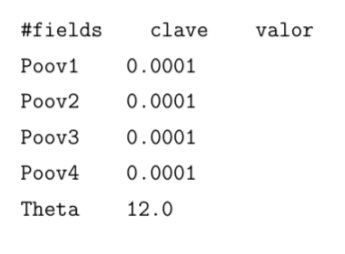
\includegraphics[width=2in]{./img/config.png}
\caption{Formato de archivo ``config''.}
\label{fig:archivoConfig}
\end{center}
\end{figure}	

La primera columna corresponde a las etiquetas que identifican los valores que se encuentran en la segunda columna. Es importante recalcar que los nombres ``Poov1'', ``Poov2'', ``Poov3'', ``Poov4'' y ``Theta'' deben ser escritos en el archivo obligatoriamente de la misma forma en la que aparecen en el ejemplo.

Por otro lado, el formato del archivo ``modeloBro.log'' es el que se muestra en la figura \ref{fig:archivoModeloBro}.

\begin{figure}[!htb]
\begin{center}
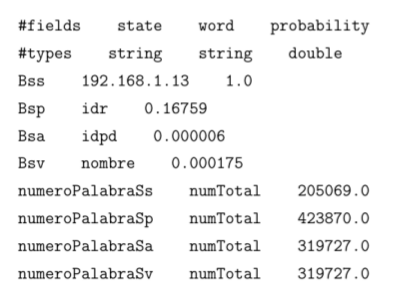
\includegraphics[width=2in]{./img/modeloBro.png}
\caption{Formato de archivo ``modeloBro.log''.}
\label{fig:archivoModeloBro}
\end{center}
\end{figure}	

La segunda columna de este archivo (``word'') corresponde al conjunto de observaciones ``O'' de cada uno de los estados, mientras que la tercera columna (``probability'') indica la probabilidad de aparición de cada palabra ($B_{S}, B_{P}, B_{A}, B_{V}$). Por otra parte, la primera columna (``state'') indica a que estado del autómata \ref{fig:ssm} pertenece cada palabra y su probabilidad de generación.

Las filas del archivo ``modeloBro.log'' que tienen en la primera columna las palabras: ``numeroPalabraSs'', ``numeroPalabraSp'', ``numeroPalabraSa'', ``numeroPalabraSv'' contienen el número de palabras que han sido procesadas por estado. Esta información será utilizada en el entrenamiento en modo ``Offline'' que será explicado en la sección.

\subsubsection*{Lectura de los Archivos}

Una vez explicado el formato de los archivos que contienen los elementos del modelo y los parámetros necesarios para realizar el cálculo y la evaluación del índice de normalidad de los URIs a evaluar se procederá a explicar el funcionamiento de las funciones encargadas de leer los archivos con la información de entrada.

Para leer dicha información se hizo uso del  ``Input Framework'' que otorga Bro como herramienta para leer archivos de entrada. La función utilizada para leer los archivos se llama ``add\_table'' y pertenece al módulo llamado ``Input''.

``add\_table'' se encarga de leer archivos de entrada y almacenar sus datos en una tabla. El formato de esta funcion es el siguiente:\\
%Extraido de : https://www.bro.org/sphinx/frameworks/input.html, https://www.bro.org/sphinx/scripts/base/frameworks/input/main.bro.html\#id-Input::add_table, https://www.bro.org/sphinx/scripts/base/frameworks/input/main.bro.html\#type-Input::TableDescription 
%
\textbf{Input::add\_table}(description: \textbf{Input::TableDescription}) : \textbf{bool} 

Donde ``\textbf{TableDescription}'' es la estructura descrita graficamente en
la figura ~\ref{fig:TableDescription} que se encuentra en el ápendice A.

\subsubsection{Evaluación de las Probabilidades de los URI}

La función ``evaluacion'' del módulo de evaluación, se encargará de hallar el  índice de anormalidad, dado un conjunto de segmentos de URI, e indicará si el mismo es anómalo o no comparándolo con el valor
de $\theta$, para luego escribir los resultados de la evaluación en un archivo de reportes del sistema. La función implementada que se encargara de realizar las tareas anteriormente descritas tiene el siguiente formato:

\textbf{evaluacion}(uriParsed: \textbf{UriSegmentado}, Bvector: \textbf{table[string,string]
of Probability}, config: \textbf{table[string] of Valor})
donde:
\begin{itemize}
\item uriParsed: es un parámetro de tipo ``UriSegmentado'' (figura \ref{fig:uriSegmentado}, ápendice A), que
almacena los segmentos del URI.
\item Bvector: es una tabla que almacena el conjunto de observaciones de cada estado (O) y el conjunto de vectores de probabilidad de las palabras observadas en cada estado, es decir, $B_{S}, B_{P}, B_{A}, B_{V}$.
\item config: Es una tabla que almacena los diferentes Poov y el valor de $\theta$.
\end{itemize}

No obstante, la tarea realizada por ``evaluacion'' fue subdividida en cuatro funciones: ``epsiloSumatoria'', ``calcularIndiceAnormalidad'',
``evaluarIndiceAnormalidad'' y ``escribirReporte''. La función ``epsiloSumatoria'' se encargará de calcular tanto el $\varepsilon_{0}$ que aparece en la expresión \ref{eq:sumB}
como la sumatoria de los logaritmos de los $p_{qtot}$ que se encuentra en la
expresión \ref{eq:Ns}.

El formato de dicha función es el siguiente:

\textbf{epsiloSumatoria}(segmentos: \textbf{UriSegmentado},
Bvector: \textbf{table[string,string] of Probability}, epsilon : \textbf{double}, estado:\textbf{string}):
\textbf{table[count] of double}

donde los parámetros de entrada serán:
\begin{itemize}
\item segmentos: es un parámetro de tipo ``UriSegmentado'' (figura \ref{fig:uriSegmentado}, ápendice A), que
almacena los segmentos del URI.
\item Bvector: es una tabla que almacena el conjunto de observaciones de cada estado (O) y el conjunto de vectores de probabilidad de las palabras observadas en cada estado, es decir, $B_{S}, B_{P}, B_{A}, B_{V}$.
\item epsilon: Valor correspondiente al Poov.
\item estado: estado del autómata que se esta evaluando (``host'',``path'',``argumentos'',
``valores'').
\end{itemize}

El parámetro de salida correspondería a una tabla que contiene dos elementos: el resultado de la suma de las probabilidades de aparición de las
palabras y la suma del los logaritmos de la probabilidad de aparición.

Por otra parte, ``calcularIndiceAnormalidad'', la encargada de calcular
el  índice de anormalidad $N_{s}$ , tiene el siguiente formato:

\textbf{calcularIndiceAnormalidad}(epsilon0: \textbf{double}, N: \textbf{double}, sumaLogaritmos: \textbf{double}) : double. Donde:

\begin{itemize}
\item epsilon0: Valor de $\varepsilon_{0}$ (expresión \ref{eq:sumB}).
\item N: Valor de ``T'' en la expresión (expresión \ref{eq:sumB}).
\item sumaLogaritmos: Suma de los logaritmos de $p_{qtot}$ que se encuentra en la expresión (expresión \ref{eq:sumB}).
\end{itemize}

El parámetro de salida de esta función será el valor del  índice de anormalidad.

La función, ``evaluarIndiceAnormalidad'' que tiene como tarea comparar el  índice de anormalidad ($N_{s}$) con el parámetro $\theta$, de la forma en que se muestra en la expresión \ref{eq:ClaseU} tiene el siguiente formato:

\textbf{evaluarIndiceAnormalidad}(theta: \textbf{double},indiceAnormalidad: \textbf{double})

donde:
\begin{itemize}
\item theta: Umbral de normalidad ($\theta$).
\item indicesAnormalidad: Índice de anormalidad.
\end{itemize}

La ultima función, ``escribirReporte'', la encargada de escribir en el archivo de reportes la información de los URIs que se han detectado como
anómalos presenta el siguiente formato:

\textbf{escribirReporte}(clasificacion: \textbf{string},
uri: \textbf{string},indiceAnormalidad: \textbf{string})

\begin{itemize}
\item clasificacion: En este campo se informa si el URI es anómalo por sobrepasar el umbral de normalidad o por estar construido de manera
incorrecta sintácticamente.
\item uri: En este campo se introduce el URI que se quiere escribir en el
archivo de salida.
\item indiceAnormalidad: Este campo corresponde al índice de anormalidad.
\end{itemize}

La función anterior fue implementada con la ayuda de las herramientas
que aporta el ``Logging Framework'' de Bro y la estructura de datos ``InfoAtaque'' (fig. ~\ref{fig:InfoAtaque}, ápendice A). La funciones del ``Framework'' utilizadas fueron: ``write'' para escribir sobre el archivo y ``create\_stream'' para crearlo. Ambas pertenecen al modulo ``LOG''. 

El formato que sigue la función ``write'' es el siguiente :

\textbf{LOG::InfoAtaque}(id: \textbf{Log::ID}, columns: \textbf{any}) : \textbf{bool}
Sus parámetros de entrada son:

\begin{itemize}
\item id: Es al ID asociado al archivo sobre el cual se va a escribir.
\item column: Registro que contiene los valores que van a ser escritos en el
archivo.
\end{itemize}

El parámetro de salida de esta función es ``verdadero'' si el archivo fue encontrado y no existieron problemas al momento de la escritura, y ``falso'' de
lo contrario.

Por otra parte, la función ``create\_stream'', esta definida de la siguiente
forma:

\textbf{LOG::create stream}(id: \textbf{Log::ID}, stream: \textbf{Log::Stream}) : \textbf{bool}

Los parámetros de entrada de la misma son:

\begin{itemize}
\item id: Es al ID asociado al archivo sobre el cual se va a escribir.
\item stream: Registro que almacenará la ruta en donde se quiere crear el
archivo y la estructura de dato que se utilizará en la escritura del
archivo.
\end{itemize}

El parámetro de salida de esta función sera ``verdadero'' si se puedo crear el
archivo y ``falso'' si es posible.


\subsection{Implementación del módulo de entrenamiento}

Como se pudo apreciar en la sección \ref{sec:entrenamiento} el modo de entrenamiento cuenta con dos modos: el modo ``Online'' y el modo ``Offline''. En esta se sección, se explicarán las funciones implementadas en cada uno de ellos.

\subsubsection{Entrenamiento ``Offline''}

El modo de entrenamiento ``Offline'', es el encargado de crear un modelo de normalidad desde cero.Esta modalidad está conformada por una
función general llamada ``entrenarOffline'', que fué subdividida en tres funciones: ``entrenamientoOffline'',
``evaluarProbabilidad'' y ``escribirArchivoOffline''.

``entrenarOffline'', será la función encargada de llamar el resto de las
funciones, necesarias para realizar el entrenamiento en modo ``Offline''. Su
formato es el siguiente:

\textbf{entrenarOffline}(segmentos: \textbf{UriSegmentado})
donde:

\begin{itemize}
\item segmentos: campo de tipo ``UriSegmentado'' (fig. \ref{fig:uriSegmentado}, ápendice A), que almacena los segmentos de un URI
\end{itemize}

Por otra parte, la función ``entrenamientoOffline'' irá observando los segmentos de los URIs de las peticiones que van llegando y contará el número de veces que cada segmento fue observado durante el entrenamiento. El formato de la misma sigue la siguiente estructura:

\textbf{entrenamientoOffline}(segmentos: \textbf{UriSegmentado}, vocabulario: \textbf{table[string] of Entrenamiento}, estado: \textbf{string})
donde:
\begin{itemize}
\item segmentos: campo de tipo ``UriSegmentado'' (fig. ~\ref{fig:uriSegmentado}, ápendice A), que almacena
los segmentos de un URI (las observaciones).
\item vocabulario: Tabla que contiene una lista de palabras y una lista de
números que corresponde al número de apariciones y probabilidad de
aparición de las misma (fig. ~\ref{fig:figEntrenamiento}, ápendice A).
\item numPalabras: Número total de apariciones de todas las palabras vistas durante el entrenamiento de un estado en concreto.
\item estado: estado del autómata que se esta entrenando (``host'', ``path'',
``argumentos'',``valores'').
\end{itemize}

La ``evaluarProbabilidad'' , encargada de tomar el resultado de las observaciones realizadas por ``entrenamientoOffline'' y calcular la probabilidad de aparición de cada uno de los segmentos (ec. \ref{eq:entrenamiento}) tiene el siguiente formato:

\textbf{evaluarProbabilidad}(vocabulario: \textbf{table[string] of Entrenamiento},
numPalabras: \textbf{double})
\begin{itemize}
\item vocabulario: Tabla que contiene una lista de palabras y una lista de
números que corresponde al número de apariciones y probabilidad de
aparición de las misma (fig. ~\ref{fig:figInfo}, ápendice A).
\item numPalabras: Número total de apariciones de todas las palabras vistas durante el entrenamiento de un estado en concreto.
\end{itemize}

Finalmente, ``escribirArchivoOffline'' toma los resultados otorgados por
``evaluarProbabilidad'' y los escribirá en un archivo de texto. El formato de
esta función es el siguiente:

\textbf{escribirArchivoOffline}(vocabulario: \textbf{table[string] of Entrenamiento}, estado: \textbf{string})
donde:
\begin{itemize}
\item vocabulario: Tabla que contiene una lista de palabras y una lista de
números que corresponde al número de apariciones y probabilidad de
aparición de las misma (fig. ~\ref{fig:figInfo}, ápendice A).
\item estado: estado al que pertenece la tabla ``vocabulario''.
\end{itemize}

\subsubsection{Entrenamiento ``Online''}

El modo de entrenamiento ``Online'', encargado de hacer modificaciones a un modelo de normalidad previamente existente fue implementado
haciendo uso de una función llamada ``entrenarOnline'' que a su vez esta
subdividida en tres funciones. Los
nombres que se les dio a estas al momento de ser implementadas fueron:
``entrenamientoOnline'',``escribirArchivoOnline''.

La función ``entrenarOnline'', cuya tarea sera llamar al resto de las funciones del entrenamiento en modo ``Online'' tiene el siguiente formato:

\textbf{entrenarOnline}(uriParsed:\textbf{segmentos::UriSegmentado})
donde:

\begin{itemize}
\item segmentos: campo de tipo ``UriSegmentado'' (fig. \ref{fig:uriSegmentado}, ápendice A), que almacena
los segmentos de un URI
\end{itemize}

Por otra parte, ``entrenamientoOnline'', encargada de calcular la probabilidad de aparición de los segmentos observados haciendo uso de de los segmentos de URI dado por ``entrenarOnline'' y el modelo de normalidad, leído por el módulo de lectura del sistema, sigue el siguiente formato:

\textbf{entrenamientoOnline}(segmentos: \textbf{UriSegmentado},
modelo: \textbf{table[string,string] of Probability}, numPalabras: \textbf{double}, state: \textbf{string})
donde:
\begin{itemize}
\item segmentos: campo de tipo ``UriSegmentado'' (fig. \ref{fig:uriSegmentado}, ápendice A), que almacena los segmentos de un URI.
\item modelo: tabla que almacena el modelo de normalidad previamente
leído.
\item numPalabras:
\item state: nombre del estado al que se le esta realizando el entrenamiento
(``host'',\\``path'',``atributos'',``valores''.
\end{itemize}

Finalmente, ``escribirArchivoOnline'', se encargará de recibir todos los
resultados obtenidos del entrenamiento para escribirlos sobre un archivo de
texto. El formato de esta función es:

\textbf{escribirArchivoOnline}(vocabulario: \textbf{table[string,string] of Probability})
donde:
\begin{itemize}
\item vocabulario: Es una tabla que almacena los resultados del entrena-
miento.
\end{itemize}


\section{Evaluación y pruebas}

En el presente sección se explicará las pruebas operativas
realizadas al sistema. Así como las bases de datos utilizadas para realizar
las misma.

\subsection{Base de datos}\label{ssec:DB}

Las bases de datos utilizadas por las pruebas fueron trazas capturadas
en servidores web. Para capturar estos paquetes de tipo HTTP los pasos a
seguir fueron los siguientes:

\begin{enumerate}
\item Se instaló una aplicación de servicio web en el ordenador.
\item Se corrió una aplicación web en la aplicación anteriormente instalada.
\item Se empezaron a hacer solicitudes a la aplicación web a tráves de otro
dispositivo. Mientras esto ocurría, ``Wireshark'' realizaba las capturas
de los paquetes de la red.
\end{enumerate}
Se obtuvo cuatro bases de datos:
\begin{itemize}
\item db1.pcap: Capturas de paquetes provenientes de las solicitudes realizadas a una aplicación web, A.
\item db2.pcap: Capturas de paquetes provenientes de la misma aplicación
web A.
\item db3.pcap: Capturas de paquetes provenientes de una aplicación web,
B.
\item db4.pcap: Capturas de paquetes descargadas de: \cite{wireshark}.
\end{itemize}

\subsection{Pruebas operativas}

A continuación, se explicaran las pruebas operativas que se les aplicaron
a las tres modalidades del sistema implementado.

\subsubsection{Modo entrenamiento ``Offline''}

Para probar el modo ``Offline'' del sistema, se tomó la base de datos \textbf{db3.pcap} explicada en la sección \ref{ssec:DB}, y se le ingresó al sistema configurado en modo ``Offline''. Una vez realizado esto, se observó el modelo de
normalidad arrojado por dicha modalidad.
En la figura \ref{fig:modeloOffline} se puede apreciar el modelo de normalidad obtenido
por la misma.

\begin{figure}[!htb]
\begin{center}
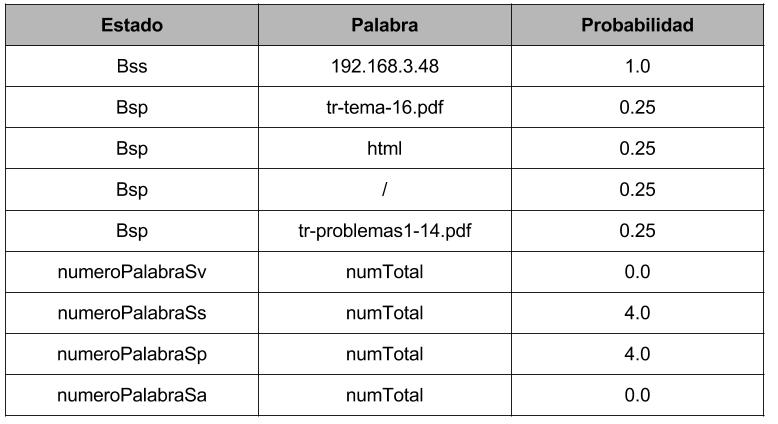
\includegraphics[width=3in]{./img/modeloOffline.jpg}
\caption{Modelo de normalidad obtenido en el modo ``Offline''.}
\label{fig:modeloOffline}
\end{center}
\end{figure}

\subsubsection{Modo entrenamiento ``Online''}

El modo ``Online'' del sistema fue probado ingresando la base de datos \textbf{db4.pcap} explicada en la sección \ref{ssec:DB} al sistema junto con el modelo mostrado en la figura \ref{fig:modeloOffline}. Una vez realizado esto, se observo la salida y se pudo verificar que, en efecto el modelo antiguo fue modificado. En la figura \ref{fig:modeloOnline} se puede apreciar la salida de esta modalidad tras la prueba realizada.

\begin{figure}[!htb]
\begin{center}
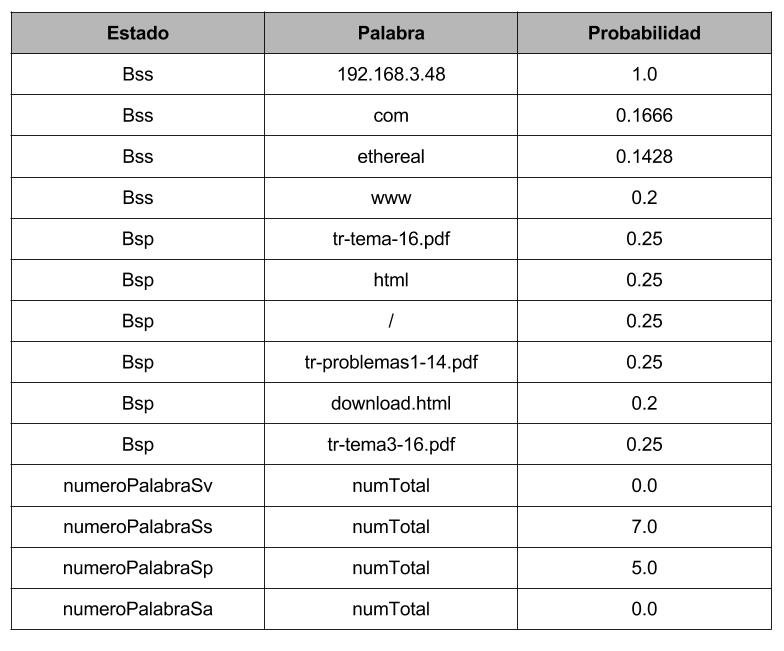
\includegraphics[width=3in]{./img/modeloOnline.jpg}
\caption{Modelo de normalidad obtenido en el modo ``Online''.}
\label{fig:modeloOnline}
\end{center}
\end{figure}

\subsubsection{Modo evaluación}

Para realizar la prueba del modo de evaluación se tomó la base de datos
\textbf{db1.pcap} para realizar un modelo de normalidad haciendo uso del modo de entrenamiento ``Offline''. De esta manera, se evaluarán las trazas que se encuentran en la base de datos, \textbf{db2.pcap} y \textbf{db3.pcap} y se observaran los resultados obtenidos.
La intención de esta prueba es comparar los  índices de anormalidad
obtenidos por la base de datos \textbf{db2.pcap} y \textbf{db3.pcap}.
Como la base de datos \textbf{db2.pcap} posee el mismo comportamiento que
el del modelo de normalidad por pertenecer a peticiones realizadas al mismo servidor, se espera que los  índices de anormalidad sean mas bajos que los obtenido por \textbf{db3.pcap}, ya que esta trazas pertenecen a peticiones que no se encuentran registradas en el comportamiento del modelo de normalidad.
En la figura \ref{fig:indicesMalos} se muestran los resultados de los  índices de anormalidad calculados cuando se evalúa la base de datos \textbf{db3.pcap}.
Se puede observar que los índices oscilan entre 25 y 36.
Por otra parte, en la figura \ref{fig:indicesBuenos} se pueden detallar los índices de anormalidad resultantes, de evaluar la base de datos \textbf{db2.pcap}.Se puede apreciar que los índices de anormalidad de la figura \ref{fig:indicesBuenos} son mas bajos que los de la figura \ref{fig:indicesMalos}. Estos resultados son los esperados, ya que \textbf{db2.pcap} no presenta incongruencias con el modelo de normalidad construido, mientras que la base de dato \textbf{db3.pcap} si. Por lo tanto es conveniente que el sistema lo catalogue como anomalías.
Un parámetro $\theta$, óptimo para esta prueba en particular, debería ser un
valor que sea menor que 25 y mayor que 18.

\begin{figure}[!htb]
\begin{center}
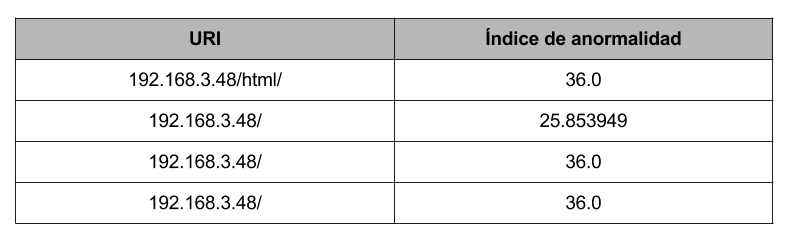
\includegraphics[width=3in]{./img/indicesMalos.png}
\caption{Índices de anormalidad obtenidos de db3.pcap.}
\label{fig:indicesMalos}
\end{center}
\end{figure}

\begin{figure}[!htb]
\begin{center}
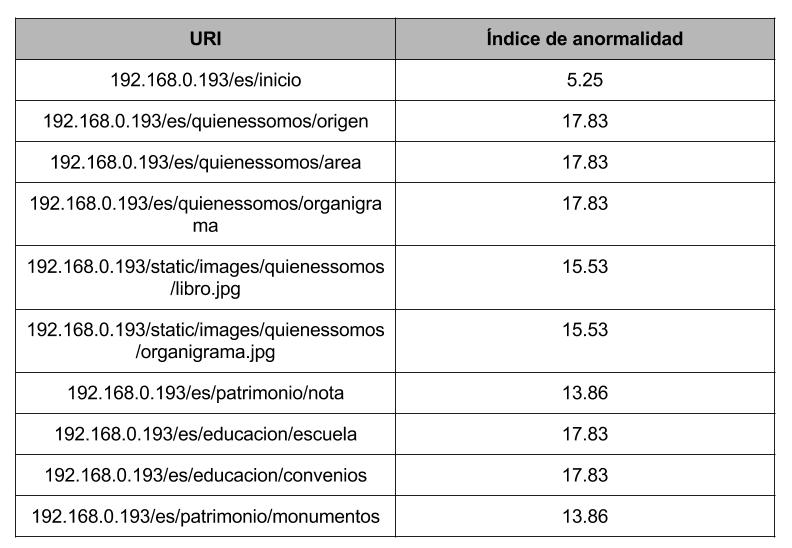
\includegraphics[width=3in]{./img/indicesBuenos.jpg}
\caption{Índices de anormalidad obtenidos de db2.pcap.}
\label{fig:indicesBuenos}
\end{center}
\end{figure}

\chapter{Conclusiones y Recomendaciones}
\label{conclusiones}
\lhead{\emph{Conclusiones y Recomendaciones}}
% Incluir recomendaciones para trabajos futuros

En este capítulo se presentarán las conclusiones y los aportes realizados por este proyecto. Así mismo, se mostrará una lista de recomendaciones, que expone un conjunto de ideas de futuras mejoras que se pueden aplicar al proyecto.

\section{Conclusiones}

En el presente proyecto se realizaron todos los objetivos planteados de manera satisfactoria. En primer lugar, se realizó un estudio de SSM (``Stochastic Structural Model'') \cite{ssm} y todos sus conceptos asociados. Una vez realizado este investigación, se diseñó una arquitectura modular del sistema, en la cual se propuso la construcción de tres módulos: uno para capturar, filtrar y segmentar los paquetes de tipo \textit{GET} del protocolo \textit{HTTP}; otro módulo que permite evaluar el índice de anormalidad de los URI y un tercer módulo para estimar los modelos de normalidad. Luego de modelar la arquitectura del sistema, se implementó cada una de las funciones del mismo haciendo uso de la herramientas y del lenguaje de ``scripting'' de Bro, con la intención de obtener un IDS basado en SSM que puede ser utilizado por servicios web en producción. Por último, se realizaron pruebas tanto funcionales como operativas. 

Los aportes realizados por este proyecto son los siguientes:

\begin{enumerate}
\item Se ha implementado un sistema que realiza detección de intrusiones en los servidores web.
\item Se ha implementado un sistema con tres funcionalidades operativas: una para realizar detección de intrusiones y dos para realizar modelos de normalidad de los servicios web.
\item Se han construido modelos de normalidad de servicios web que podrían ser utilizados para la detección de intrusiones.
\end{enumerate}

\section{Recomendaciones}

\begin{enumerate}
\item Calcular de manera experimental los valores óptimos de $\theta$ y los de probabilidad fuera de vocabulario que generen la menor cantidad posible de falsos positivos, haciendo uso de bases de datos mas extensas.
\item Agregarle al IDS un conjunto de firmas de ataques conocidos aplicando la técnica propuesta en \cite{firmas}.
\item Probar el sistema en un entorno de producción.
\item Ampliar el sistema para que funcione en otros protocolos de la red.
\end{enumerate}

% El estilo de la bibliografía es AAAI, definido en el archivo aaai.bst.
\begin{thebibliography}{99}
\bibitem{pwc} 
PWC: PricewaterhouseCoopers,
\\\texttt{\url{https://www.pwc.com/gx/en/services/advisory/forensics/economic-crime-survey/cybercrime.html}}

\bibitem{salario}
Walters R. (2017), \textit{Salary Survey}, disponible en: \url{https://www.robertwalters.co.uk/content/dam/salary-survey-2017.pdf?webSyncID=6d3bc948-9837-8e7b-91d2-a51713c993b7&sessionGUID=0b156ce4-a2a8-3d94-8cd0-15640ae068ac}

\bibitem{IDSdef} Sundar Rajan, S., \& Krishna Cherukuri, V. (2017).\textit{An Overview of Intrusion Detection Systems }. Disponible en: \url{http://www.idt.mdh.se/kurser/ct3340/ht09/ADMINISTRATION/IRCSE09-submissions/ircse09_submission_18.pdf}

\bibitem{IDSimportance} R,K. \& Indra, A.(2010) \textit{Intrusion Detection Tools and Techniques --
A Survey. International Journal Of Computer Theory An Enginering}, 901-906. http://dx.doi.org/10.7763/ijcte.2010.v2.260.

\bibitem{ugr} Granada y la Universidad. Disponible en: \url{https://www.ugr.es/universidad/organizacion/granada-y-la-universidad}

\bibitem{etsii} La Escuela de Informática y Telecomunicación. Disponible en: \url{https://etsiit.ugr.es/pages/escuela}

\bibitem{ugrMV} Misión y Visión de la Universidad de Granada. Disponible en: \url{http://www.ugr.es/~rhuma/sitioarchivos/noticias/MisionVision.pdf}

\bibitem{etsiiDepart} Departamentos que imparten docencia en la ETSIIT. Disponible en: \url{https://etsiit.ugr.es/pages/escuela/departamentos}

\bibitem{IDS}
H.   Debar (2000), \textit{An Introduction to Intrusion-Detection Systems},  IBM   Research,   Zurich   Research   Laboratory,Ruschlikon, Switzerland.

\bibitem{rfcHTTP}
RFC 7230

\bibitem{rfcURI}
RFC 3986

\bibitem{automata}
Linz P. (2012) \textit{An Introduction to FORMAL LANGUAGE an AUTOMATE}, quinta edición, pp 36.

\bibitem{automata2}
Mishra K.L.P. , Chandrasekaran N. (2008), \textit{THEORY OF COMPUTER SCINCE Automata, Language and Computation},tercera edición, pp 71-72.

\bibitem{automataFinito}
V. Aho A., S. Lam M., Sethi R., D. Ullman J. (2007),\textit{Compilers, Principles, Techniques, \& Tools}, segunda edición,pp 147-150.

\bibitem{markov}
Ching W., Ng M. K. (2006), \textit{Markov Chains: Models, Algorithms and Applications}, pp 1-4.

\bibitem{ejemploMarkov}
Haggstrom (2002) \textit{Finite Markov Chains and Algorithmic Applications}, Lon-
don Mathematical Society, Student Texts 52, Cambridge University Press,Cambridge, U.K.

\bibitem{ssm}
Pedro García-Teodoro.; Jesús E. Díaz-Verdejo; Juan M. Tapiador; Rolando Hernandez-Salazar
Automatic Generation of HTTP Intrusion Signatures by Selective Identification of Anomalies
Computers \& Security, Vol. 55, pp. 159-174, 2015, ISSN: 0167-4048 

\bibitem{tesisMexico}
Rolando Salazar Hernández, Sistema de detección de intrusos mediante modelado de URI. Tesis doctoral. Universidad de Granada. Director: Jesús E. Díaz Verdejo, 02/02/2016

\bibitem{GitHub} \textit{About - GitHub}. Disponible en: \url{https://github.com/about}

\bibitem{Git} \textit{GitHub Glossary}. Disponible en: \url{https://help.github.com/articles/github-glossary/}

\bibitem{wireshark1} \textit{Wireshark - about}. Disponible en : \url{https://www.wireshark.org/about.html}

\bibitem{wireshark2} \textit{Wireshark - docs}. Disponible en: \url{https://www.wireshark.org/docs/wsug_html_chunked/ChapterIntroduction.html}

\bibitem{Bro}
\textit{Bro Introduction}, disponible en : \url{https://www.bro.org/sphinx/intro/index.html}

\bibitem{httpKross}
Kurose, J. F., \& Ross, K. W. (2013). \textit{Computer networking: a top-down aproach}. Pearson

\bibitem{Cormen} Cormen H. C., Leiserson E. C., Rivest L. R., Stein C. (2009).Introduction to algorithms, tercera edición, pp 153-155.

\bibitem{wireshark} Capturas de ejemplo de “Wireshark”. Disponible en:  \url{https://wiki.wireshark.org/SampleCaptures?action=AttachFile&
do=view&target=http.cap}

\bibitem{firmas} García-Teodoro P., Díaz-Verdejo J.E., Tapiador J.E., Salazar-Hernández R. (2015) \textit{Automatic generation of HTTP intrusion of anomalies}

\end{thebibliography}

\label{Bibliography}
\bibliography{bibliografia}
\lhead{\emph{Bibliografía}}
%\bibliographystyle{ieeetr}
\addtocontents{toc}{\vspace{2em}}

\begingroup
    \setstretch{1}
    \bibliography{referencias}
\endgroup

\glsaddall
\printglossary

% Apéndices
\appendix
\chapter{@nombreApendice}
\label{apendiceA}
\lhead{Apéndice A. \emph{@nombreApendice}}

% En los apéndices se incluye cualquier información que no sea esencial para la
% comprensión básica del trabajo, pero provea ejemplos y casos de estudio
% extendidos que permitan un análisis más exhaustivo.

\section{@sección}


\subsection{@subsección}


``Saludo''.

\chapter{Pruebas Funcionales Realizadas}
\label{apendiceB}
\lhead{Apéndice B. \emph{Pruebas Funcionales Realizadas}}

\section*{Pruebas funcionales}

En esta sección se explicarán las pruebas funcionales aplicadas a cada
una de la funciones construidas en el sistema.

\subsection*{Filtro HTTP/GET}

Para probar el filtro de tipo HTTP/GET se tomó la base de datos,
\textbf{db1.pcap}, que contiene tanto paquetes HTTP/GET, como paquetes correspondientes a la sesión HTTP. La prueba consistió en pasarle a la función construida la base de datos de paquetes para que esta imprimiera los URIs de las peticiones HTTP/GET que estuviesen contenidas en la misma. En la
figura \ref{fig:filtroHTTP} se muestra un esquema de la prueba que se realizó.

\begin{figure}[!htb]
\begin{center}
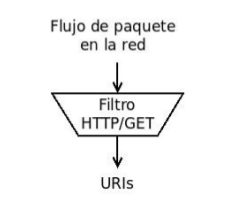
\includegraphics[width=2in]{./img/filtroHTTP.png}
\caption{Esquema de pruebas realizadas al filtro HTTP/GET.}
\label{fig:filtroHTTP}
\end{center}
\end{figure}

\subsection*{Lectura de Archivos}

La lectura de los archivos es de suma importancia, ya que el sistema utiliza un modelo de normalidad y un conjunto de parámetros que se introducen
al mismo a tráves de archivos.
La manera en la que se probó esta función consistió en leer ambos archivos de textos necesarios por el sistema: ``config'' y ``modeloBro.log'' y luego se imprimieron las tablas resultantes de la lectura de los mismos.
En la figura \ref{fig:configFile}, se puede observar el archivo ``config'' que leerá la función de lectura del sistema y en la figura \ref{fig:configResult}, se puede apreciar la forma en la
que la misma almacenó los datos en la tabla correspondiente.
Por otra parte, en la figura \ref{fig:modelFile}, está el archivo ``modeloBro.log'' que fué utilizado en la prueba realizada, mientras que en la figura \ref{fig:modelResult} se muestra el resultado arrojado por la misma.

\begin{figure}[!htb]
\begin{center}
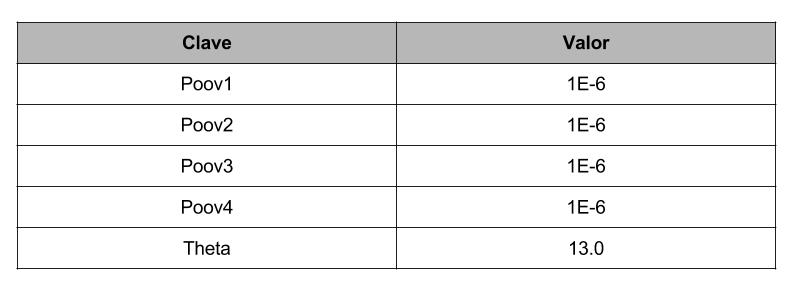
\includegraphics[width=3in]{./img/configFile.jpg}
\caption{Archivo ``config''.}
\label{fig:configFile}
\end{center}
\end{figure}

\begin{figure}[!htb]
\begin{center}
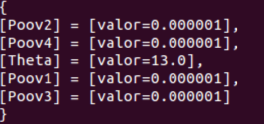
\includegraphics[width=3in]{./img/tablaConfig.png}
\caption{Tabla que contiene información del archivo ``config''.}
\label{fig:configResult}
\end{center}
\end{figure}

\begin{figure}[!htb]
\begin{center}
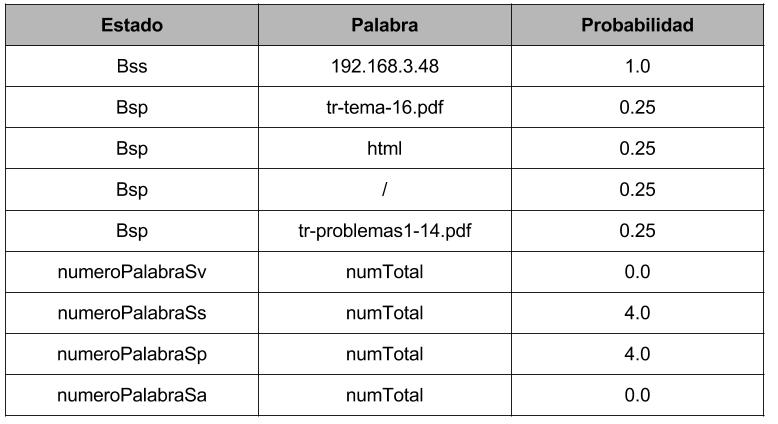
\includegraphics[width=3in]{./img/modeloOffline.jpg}
\caption{Archivo ``modeloBro.log''.}
\label{fig:modelFile}
\end{center}
\end{figure}

\begin{figure}[!htb]
\begin{center}
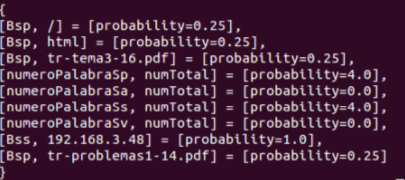
\includegraphics[width=3in]{./img/tablaModeloBro.png}
\caption{Tabla que contiene información del archivo ``modeloBro.log''.}
\label{fig:modelResult}
\end{center}
\end{figure}

\subsection*{Módulo de Segmentación}

Como se mencionó en los secciones anteriores, el modulo de segmentación
cuenta con dos funciones principales: la función de normalización y la de
segmentación. A continuación se mostrará la manera en la que se probó cada una de las funciones.

\subsection*{Función de Normalización}

Las pruebas realizadas a la función de normalización consistió en realizar una lista de URIs sin normalizar, ingresarlos como parámetros a la función y observar los resultados arrojados por la misma.
La lista de URIs utilizados en esta prueba se pueden observar en la figura \ref{fig:uriSinNorm}. Por otra parte, los resultados arrojados por la misma se muestran en la
figura \ref{fig:uriNorm}.

\begin{figure}[!htb]
\begin{center}
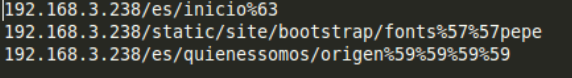
\includegraphics[width=3in]{./img/uriSinNorm.png}
\caption{URIs sin normalizar.}
\label{fig:uriSinNorm}
\end{center}
\end{figure}

\begin{figure}[!htb]
\begin{center}
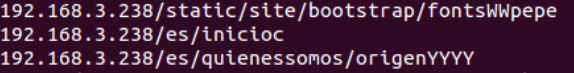
\includegraphics[width=3in]{./img/uriNorm.png}
\caption{URIs normalizados.}
\label{fig:uriNorm}
\end{center}
\end{figure}


\subsection*{Función de Segmentación}

La pruebas realizadas a la función de segmentación, consistieron en ingresarle un conjunto de URIs a la misma y observar la manera en la que
esta los segmentaba.

\subsection*{Módulo de Entrenamiento}
\subsubsection*{Modo ``Offline''}
Como se pudo observar en los secciones anteriores, el módulo de entrenamiento esta conformado por una función, ``entrenarOffline'', que que se
encarga de hacer la llamada a función de: ``entrenamientoOffline'', ``evaluarProbabilidad'', ``escribirArchivoOffline''.
Para probar la función, ``entrenamientoOffline'', se construyeron una serie de datos de tipo ``UriSegmentado'' (fig. \ref{fig:uriSegmentado}), provenientes de la base de datos \textbf{db3.pcap} y le fueron pasados como parámetro de entrada a la misma. Una vez procesados los datos, se observó la salida de la misma para verificar la correctitud.

Por otra parte, para probar la función ``evaluarProbabilidad'', se tomaron los resultados arrojados por ``entrenamientoOffline'' y se
observó el resultado que arrojaba la misma. 

La prueba que se le realizó a ``escribirArchivoOffline'', consistió en tomar el resultado arrojado por ``evaluarProbabilidad'' y observar el
archivo de salida que escribía dicha función. 

\subsubsection*{Modo ``Online''}
Al igual que el modo ``Offline'', el modo ``Online'' esta conformado por
una función,``entrenarOnline'', que se encarga de hacer la llamada a función
del resto:``entrenamientoOnline'',``escribirArchivoOnline''
Las pruebas de ``entrenamientoOnline'' consistieron en darle un modelo de normalidad y un conjunto de estructura
de tipo ``UriSegmentado'' y observar la salida que arrojaba la misma.

Para probar la función ``escribirArchivoOnline'', se tomó el resultado arrojado por ``entrenamientoOnline'' y se observó el archivo de salida escrito por la misma.
\subsubsection*{Módulo de Evaluación}

El modulo de evaluación consta de una función general, llamada ``evaluacion'' que se encarga de hacer la llamada a función de: ``epsiloSumatoria'',
``calcularIndiceAnormalidad'', ``evaluarIndiceAnormalidad'' y ``escribirReporte'', que a su vez se encargan de realizar el trabajo del módulo de evaluación.
Para probar la función ``epsiloSumatoria'', se ingresó un conjunto de datos de tipo de tipo ``UriSegmentado'', un modelo de normalidad previamente leído, un valor para el epsilon, y un conjunto de estado del autómata para observar los resultados que arrojaba la misma.
Para la prueba de la función ``calcularIndiceAnormalidad'', se tomaron
los resultados proporcionados por la función ``epsiloSumatoria'' y se observará el resultado obtenido.

Tanto los resultados obtenidos por ``epsiloSumatoria'' por ``calcularIndiceAnormalidad'' fueron verificados calculando de manera manual los valores
que estas funciones calculan, haciendo uso de las expresiones correspondientes.
Las pruebas de la función ``evaluarIndiceAnormalidad'' consistieron en
darle un  índice de anormalidad y un valor del parámetro $\theta$, como los que
se muestran en la figura \ref{fig:archivoConfig} y verificar si la misma clasificaba de manera adecuada.
Finalmente, para realizar la prueba de ``escribirReporte'' se le pasó una serie de URIs pertenecientes a la base de datos \textbf{db1.pcap}. Una vez realizado
esto, se observó el archivo de salida escrito por dicha función.

%\addtocontents{toc}{\vspace{2em}}
%\backmatter

\end{document}
